\chapter{Results and interpretations}
\label{chap:results}

The analysis described in the previous Chapters has been carried out
on the $12.9\pm0.8~\ifb$ dataset that was introduced in
Sec.~\ref{sec:dataset}, the results are described in this Chapter. The
\SM backgrounds have been predicted using the likelihood fit discussed
in Sec.~\ref{sec:likelihood}. The data has then been compared to the expected
background yields and limits are set on the production of an array of
different \SUSY models. This result has been released publicly
at \cite{CMS-PAS-SUS-16-016}.

%%%%%%%%%%%%%%%%%%%%
\section{Results}

The total predicted \SM yields for each of the (\HT,\nj,\nb) bins,
integrated over the \MHT dimension, are shown in
Figs.~\ref{fig:mono},~\ref{fig:asym} and \ref{fig:sym} for the
monojet, asymmetric and symmetric jet categories respectively. In the
top panel of each figure, the data counts with a representative
statistical uncertainty are shown as black circles with error bars.
The coloured histogram shows the result of the \SM background
prediction with the \TF methods described in
Chapter~\ref{chap:backgroundPred}, the uncertainty of this prediction
is represented with a shaded box (CR-only fit uncertainty). The
predictions are split into the \znunu, \QCD multijet and other
remaining \SM backgrounds. On the bottom panel of each plot, the
significance of the deviation of the data from the predicted \SM
background is plotted. The red circles show the deviation of the
control region only background fit (Eq.~\ref{eq:controlLikelihood}),
while the blue circles show the deviation of the fit that includes the
signal region (Eq.~\ref{eq:total_likelihood}). The deviation is
represented as a \emph{pull} that is defined as the number of observed
events, minus the number of predicted events, divided by the $1\sigma$
uncertainty.

Along with the background prediction in each of the (\HT,\nj,\nb)
categories, simulation is used to predict the \MHT shapes. The result
of this prediction for a series of representative bins is shown in
Fig.~\ref{fig:mht-templates}. The data yields and statistical errors
are displayed by the black markers. The \MHT shape taken from
simulation normalised based on the results from the control region
only fit is displayed as the green histogram.

Overall, no significant deviation from the \SM backgrounds is observed
in the data. The results are well described by a \SM-only hypothesis.
There are a few large pulls, $\sim 3\sigma$, that are observed in the
control-region only fit. However, after a fit including the signal
region is carried out the pulls are significantly reduced. This
suggests that such effects are properly covered by systematic
uncertainties.

\begin{figure}[!htb]
  \begin{center}
    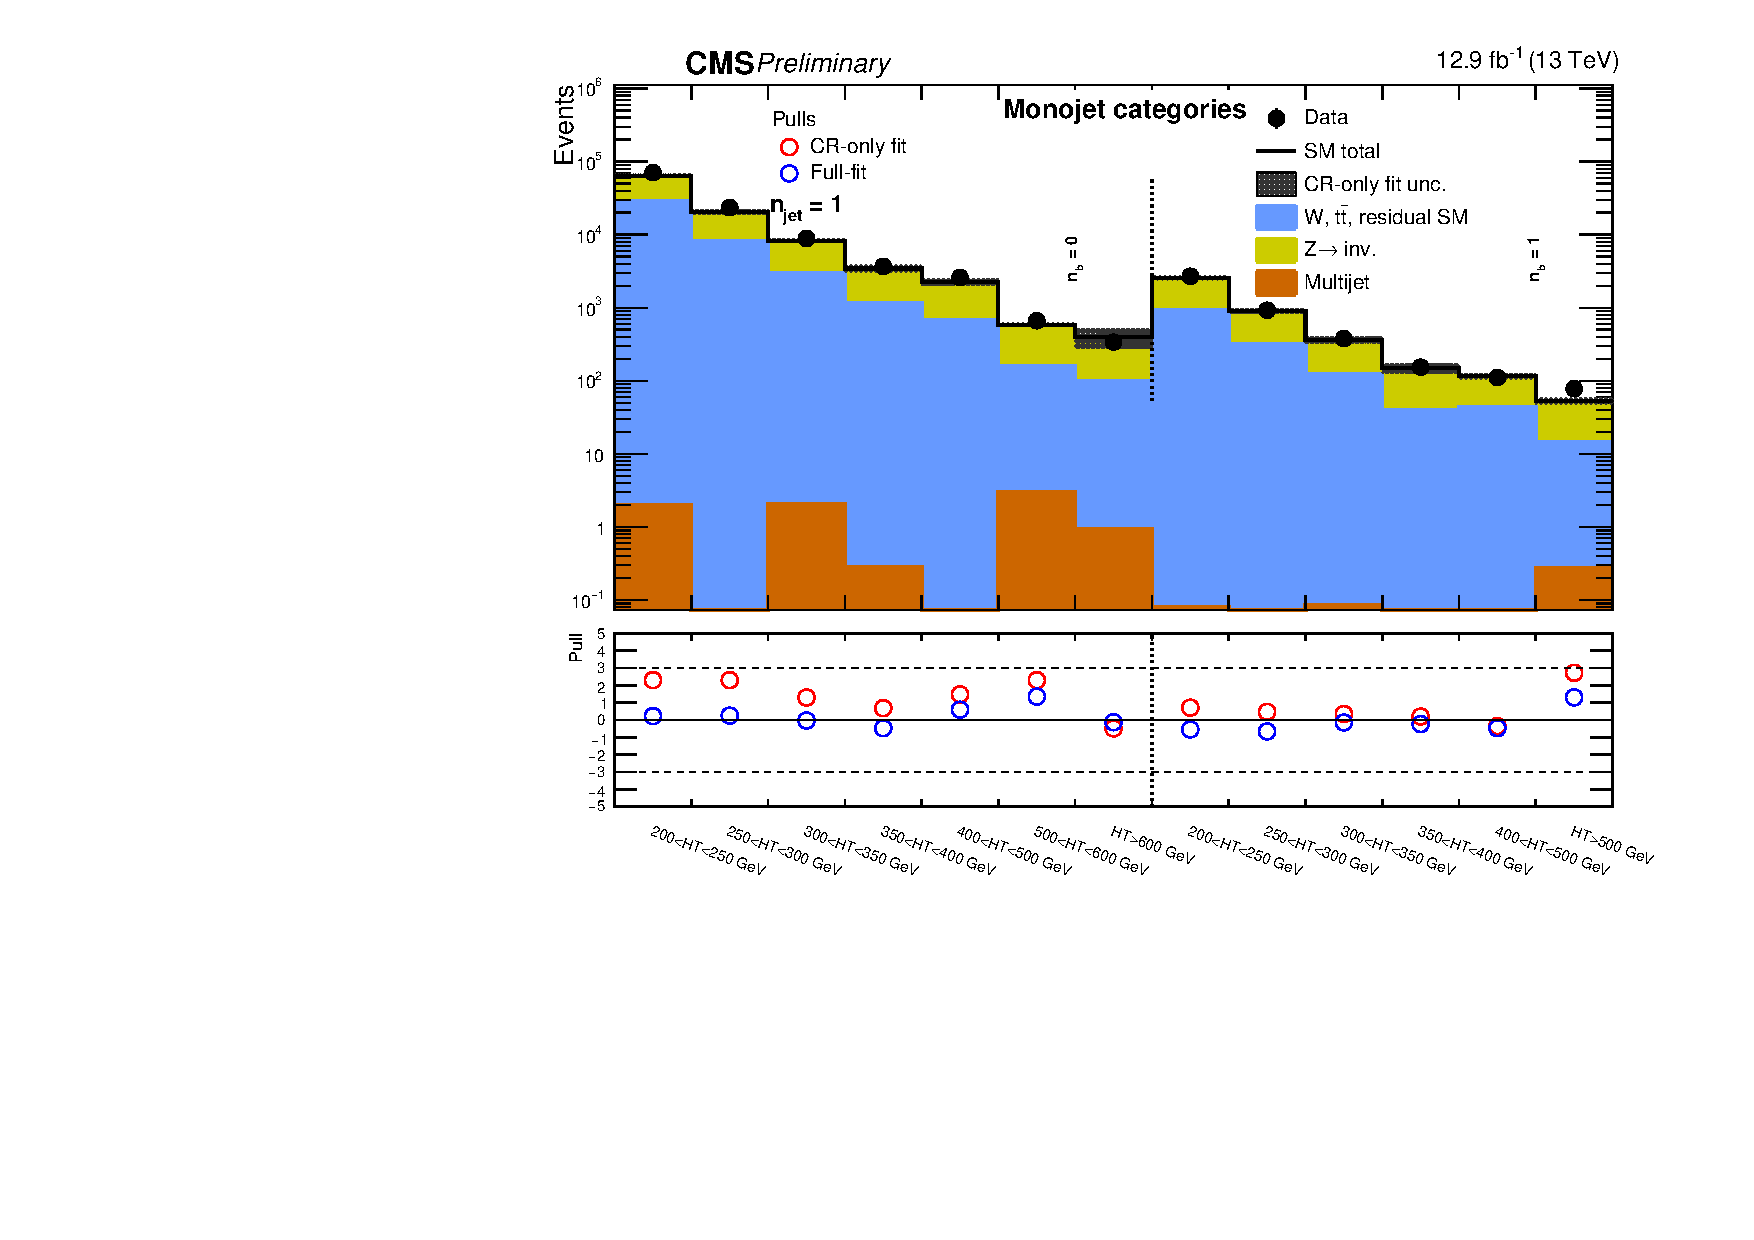
\includegraphics[width=0.9\textwidth]{figs/analysis/results/summaryPlot_Monojet_prefit_overlay_fit_b}
    \caption{The total event yields in data (solid black circles)
      and the \SM expectations with their associated uncertainties (black
      histogram with shaded band) as a function of
      \nb and \HT for the monojet topology ($\njet = 1$) in the
      signal region. Under this is the significance of deviations
      (pulls) observed in data with respect to the \SM expectations
      from the fit with only the control regions (red circles) and a
      full fit including the signal region (blue circles).}
    \label{fig:mono}
  \end{center}
\end{figure}

\begin{figure*}[!htb]
  \begin{center}
    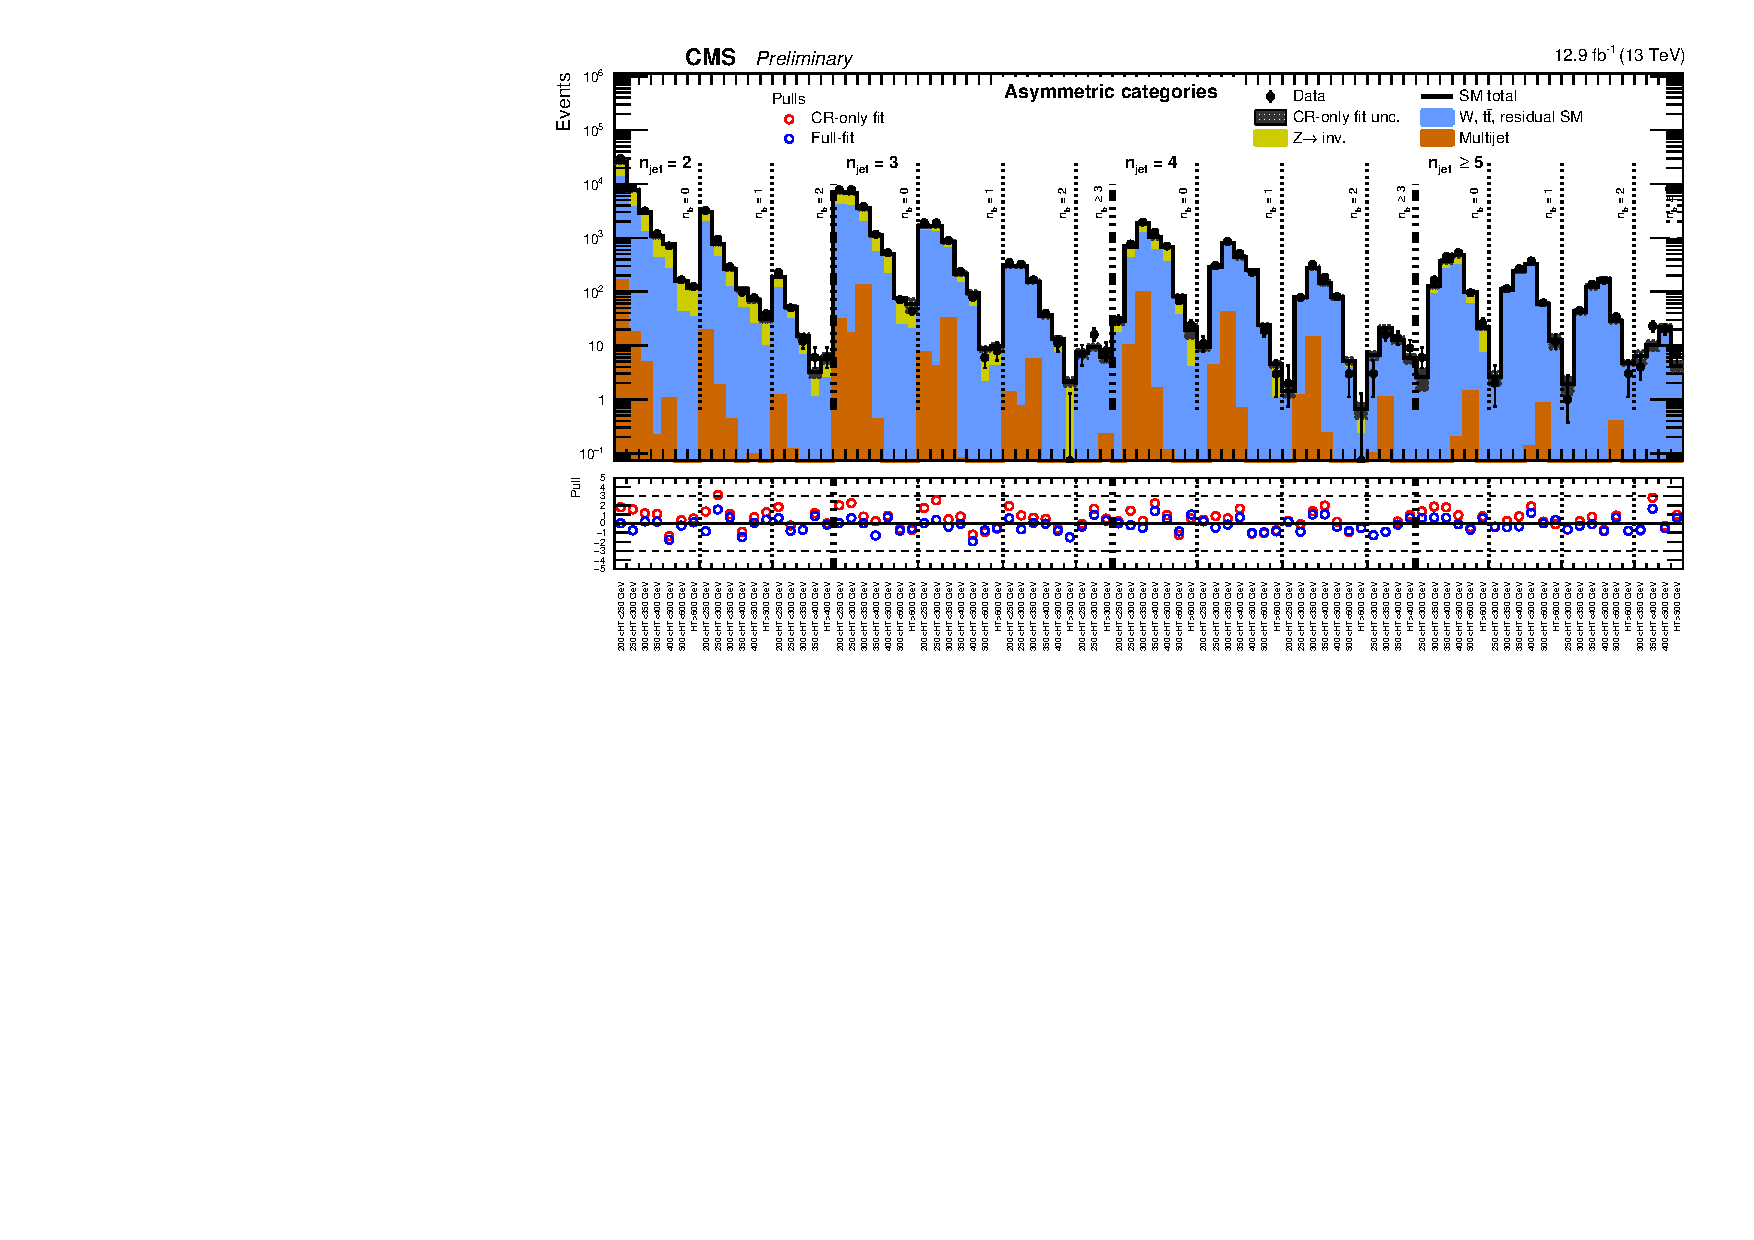
\includegraphics[angle=90,width=0.7\textwidth]{figs/analysis/results/summaryPlot_Asymmetric_prefit_overlay_fit_b}
    \caption{The total event yields in data (solid black circles)
      and the \SM expectations with their associated uncertainties (black
      histogram with shaded band) integrated over \MHT as a function of
      \nj,\nb and \HT for the asymmetric topology in the
      signal region. Under this is the significance of deviations
      (pulls) observed in data with respect to the \SM expectations
      from the fit with only the control regions (red circles) and a
      full fit including the signal region (blue circles).}
    % \caption{(Top panel) Event yields observed in data (solid circles)
    %   and SM expectations with their associated uncertainties (black
    %   histogram with shaded band) from a CR-only fit, integrated over
    %   \MHT, as a function of \njet, \nb, and \scalht for the
    %   asymmetric topology in the signal region. (Bottom panel). The
    %   significance of deviations (pulls) observed in data with respect
    %   to the SM expectations from the CR-only (red circles) and full
    %   fit (blue circles). The pulls are indicative only and cannot be
    %   considered independently.}
    \label{fig:asym}
  \end{center}
\end{figure*}

\begin{figure*}[!htb]
  \begin{center}
    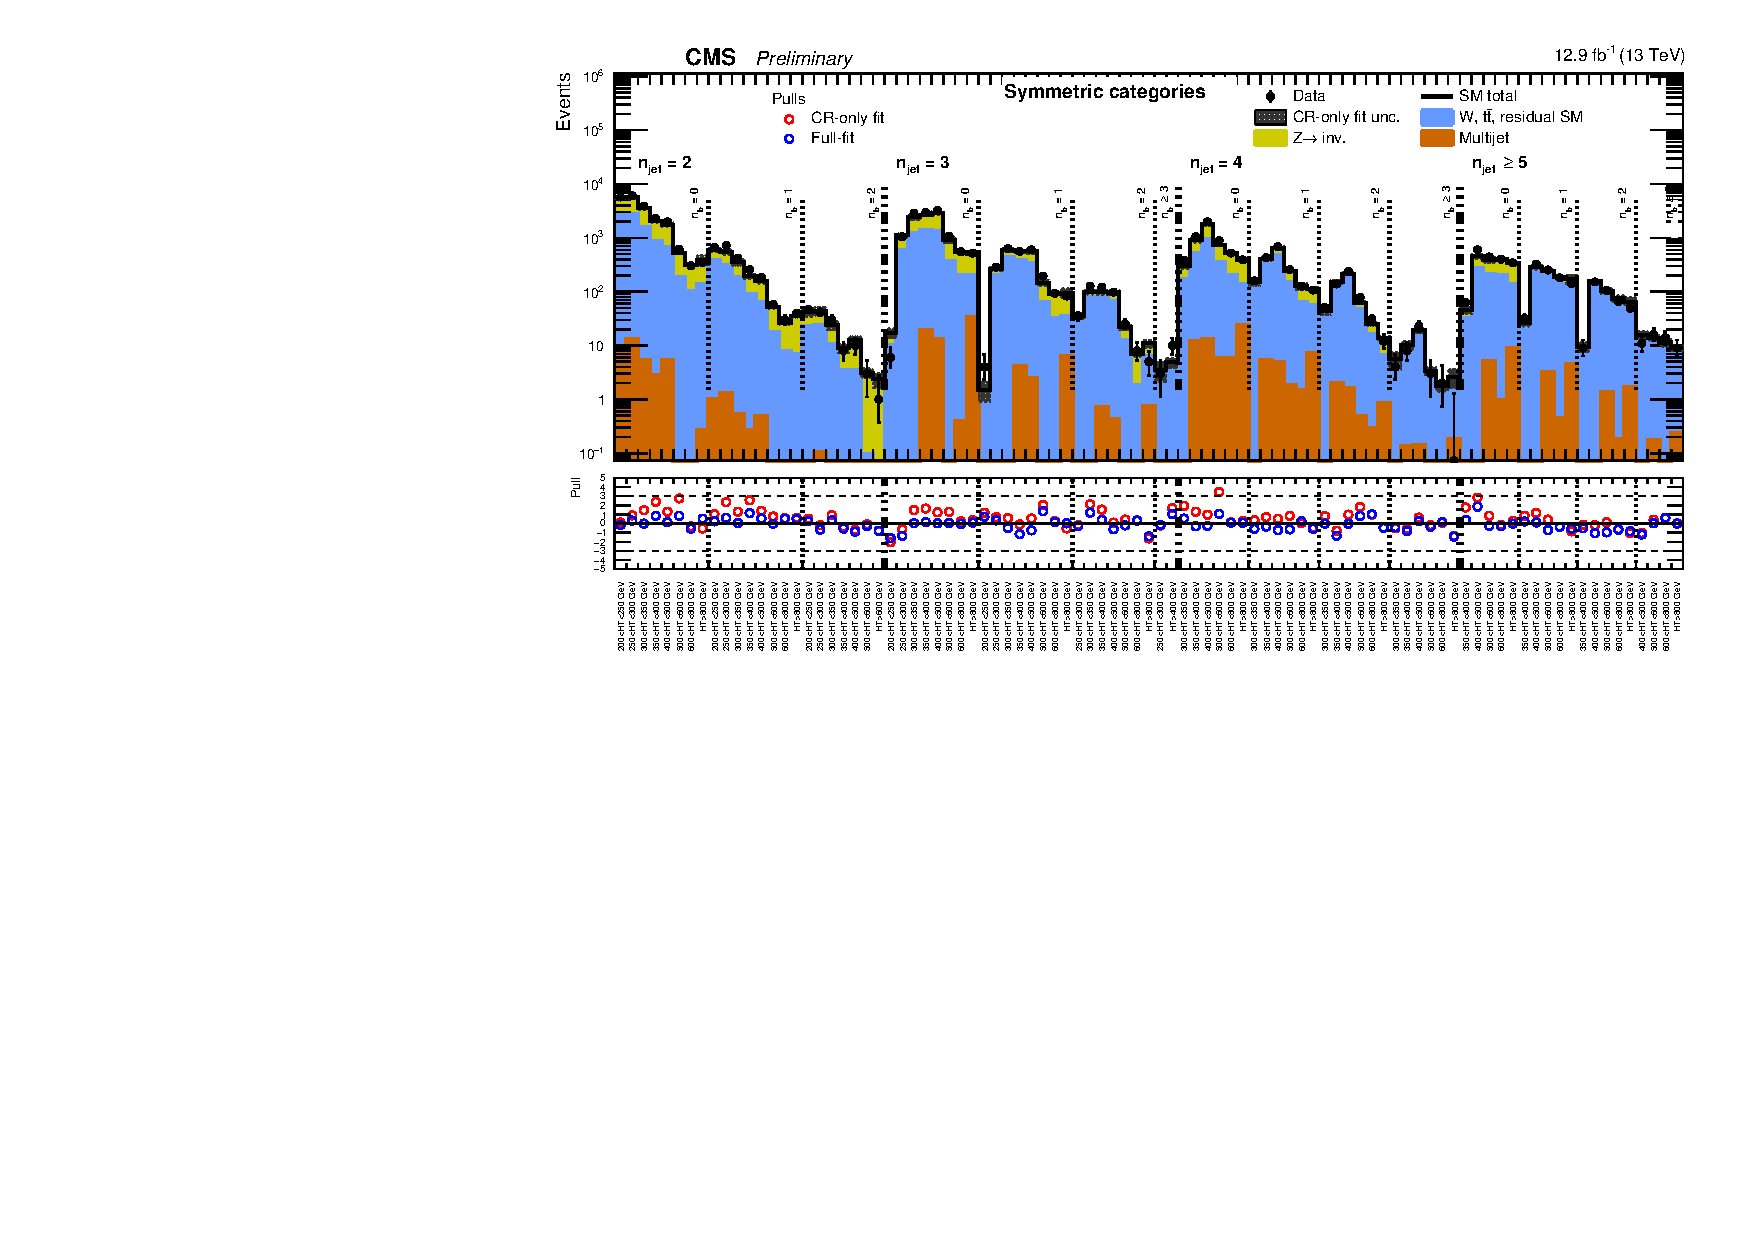
\includegraphics[angle=90,width=0.7\textwidth]{figs/analysis/results/summaryPlot_Symmetric_prefit_overlay_fit_b}
    % \caption{(Top panel) Event yields observed in data (solid circles)
    %   and SM expectations with their associated uncertainties (black
    %   histogram with shaded band) from a CR-only fit, integrated over
    %   \MHT, as a function of \njet, \nb, and \scalht for the
    %   symmetric topology in the signal region. (Bottom panel). The
    %   significance of deviations (pulls) observed in data with respect
    %   to the SM expectations from the CR-only (red circles) and full
    %   fit (blue circles). The pulls are indicative only and cannot be
    %   considered independently.}
    \caption{The total event yields in data (solid black circles)
      and the \SM expectations with their associated uncertainties (black
      histogram with shaded band) integrated over \MHT as a function of
      \nj,\nb and \HT for the symmetric topology in the
      signal region. Under this is the significance of deviations
      (pulls) observed in data with respect to the \SM expectations
      from the fit with only the control regions (red circles) and a
      full fit including the signal region (blue circles).}
    \label{fig:sym}
  \end{center}
\end{figure*}

\begin{figure*}[!tbhp]
  \begin{center}
  \subfloat[Symmetric topology, medium \HT, low \nj]{
    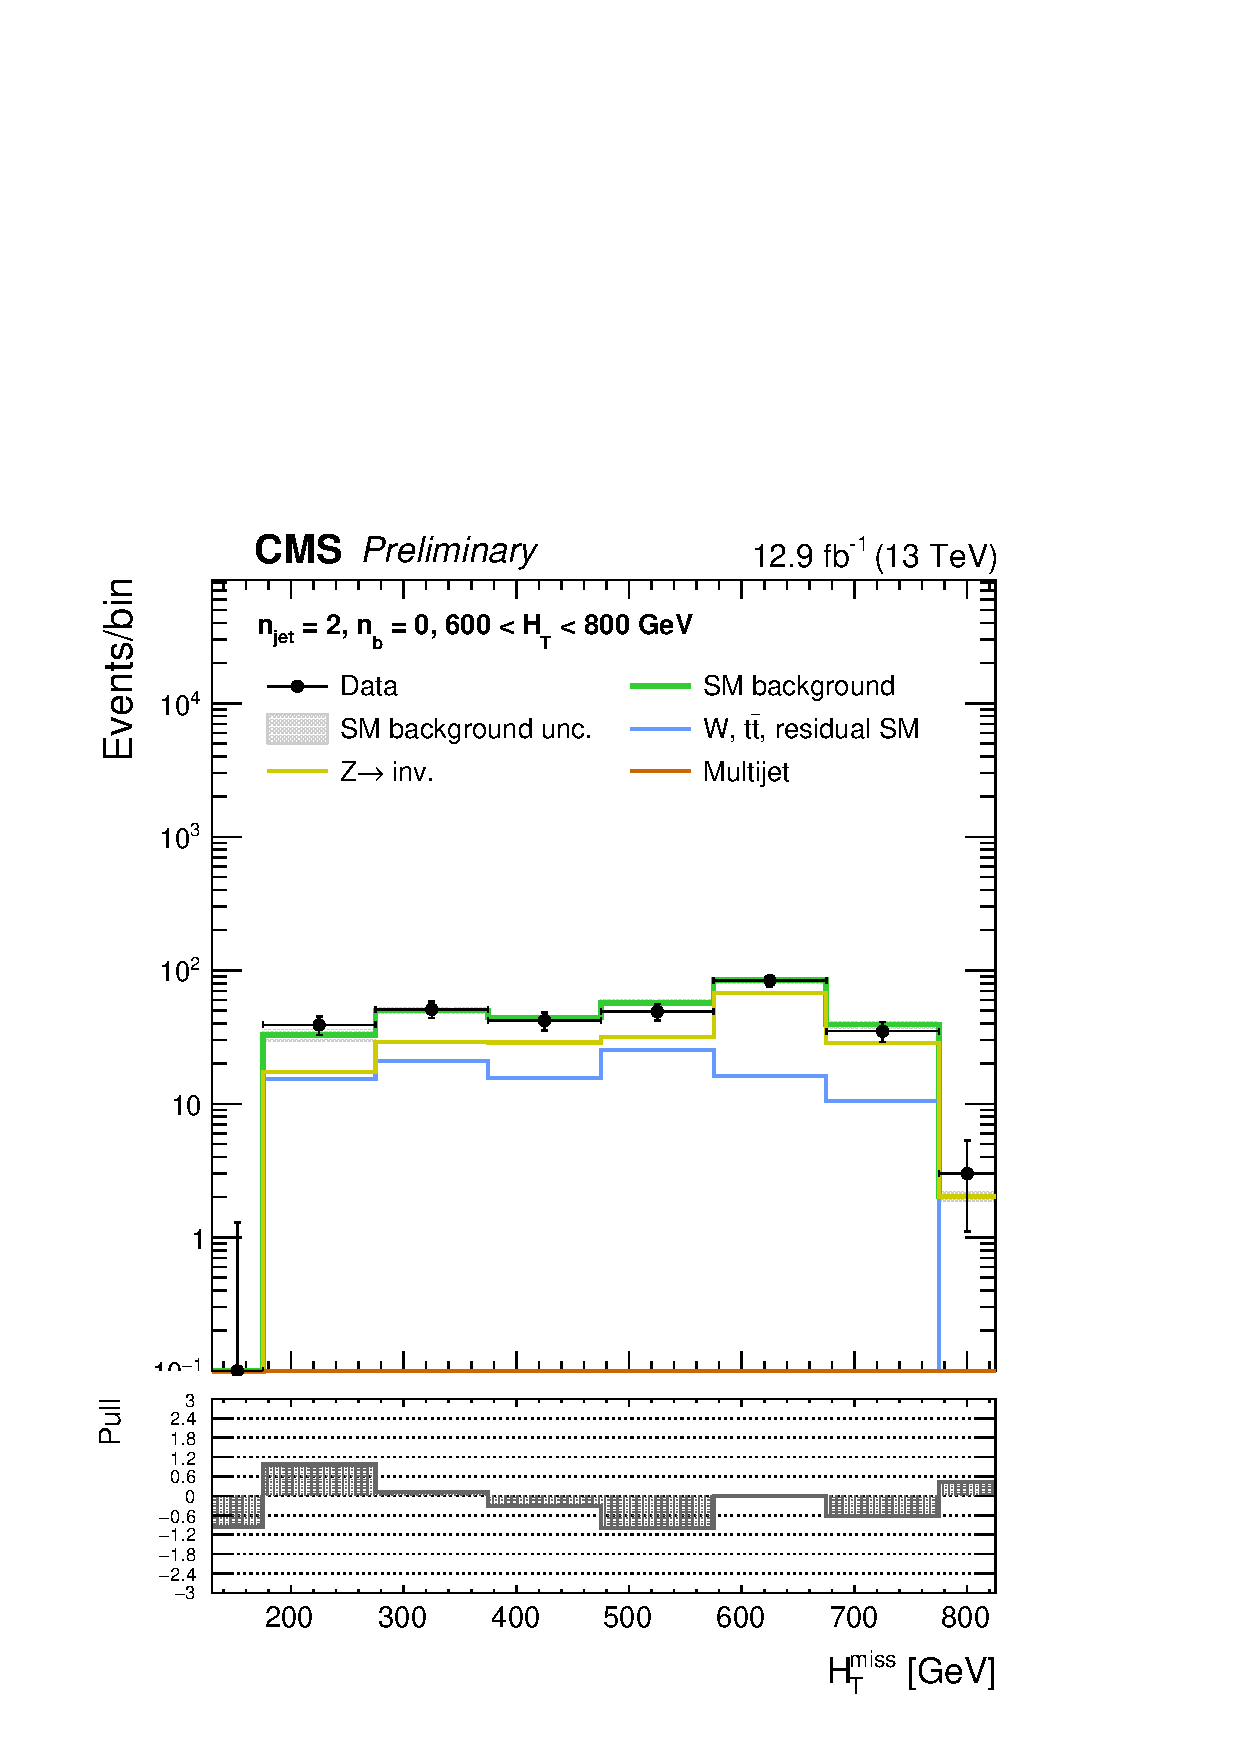
\includegraphics[width=0.49\textwidth]{figs/analysis/results/mhtShape_eq0b_eq2j_600_800_fit_b.pdf}
    }~~
  \subfloat[Asymmetric topology, low \HT]{
    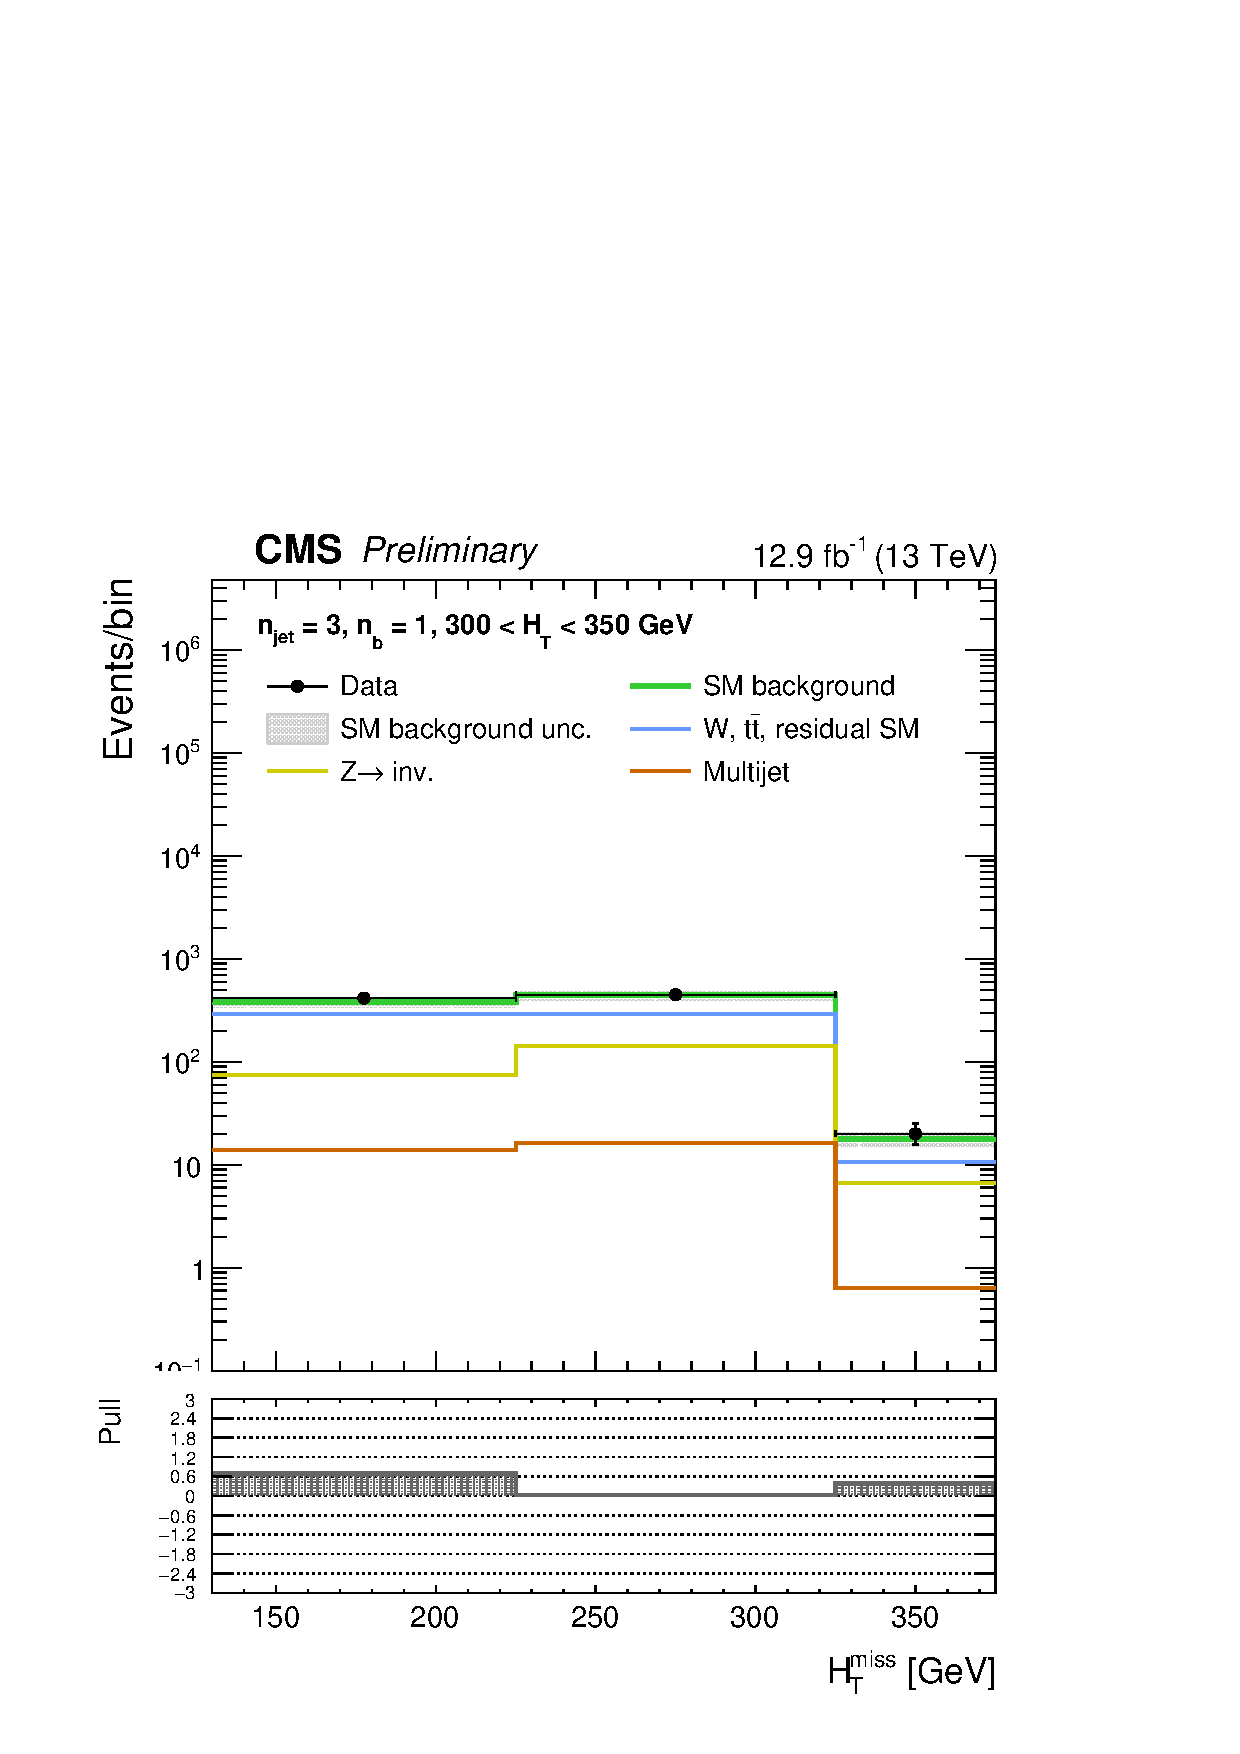
\includegraphics[width=0.49\textwidth]{figs/analysis/results/mhtShape_eq1b_eq3a_300_350_fit_b.pdf}
    }\\
  \subfloat[Symmetric topology, high \nj and \HT]{
    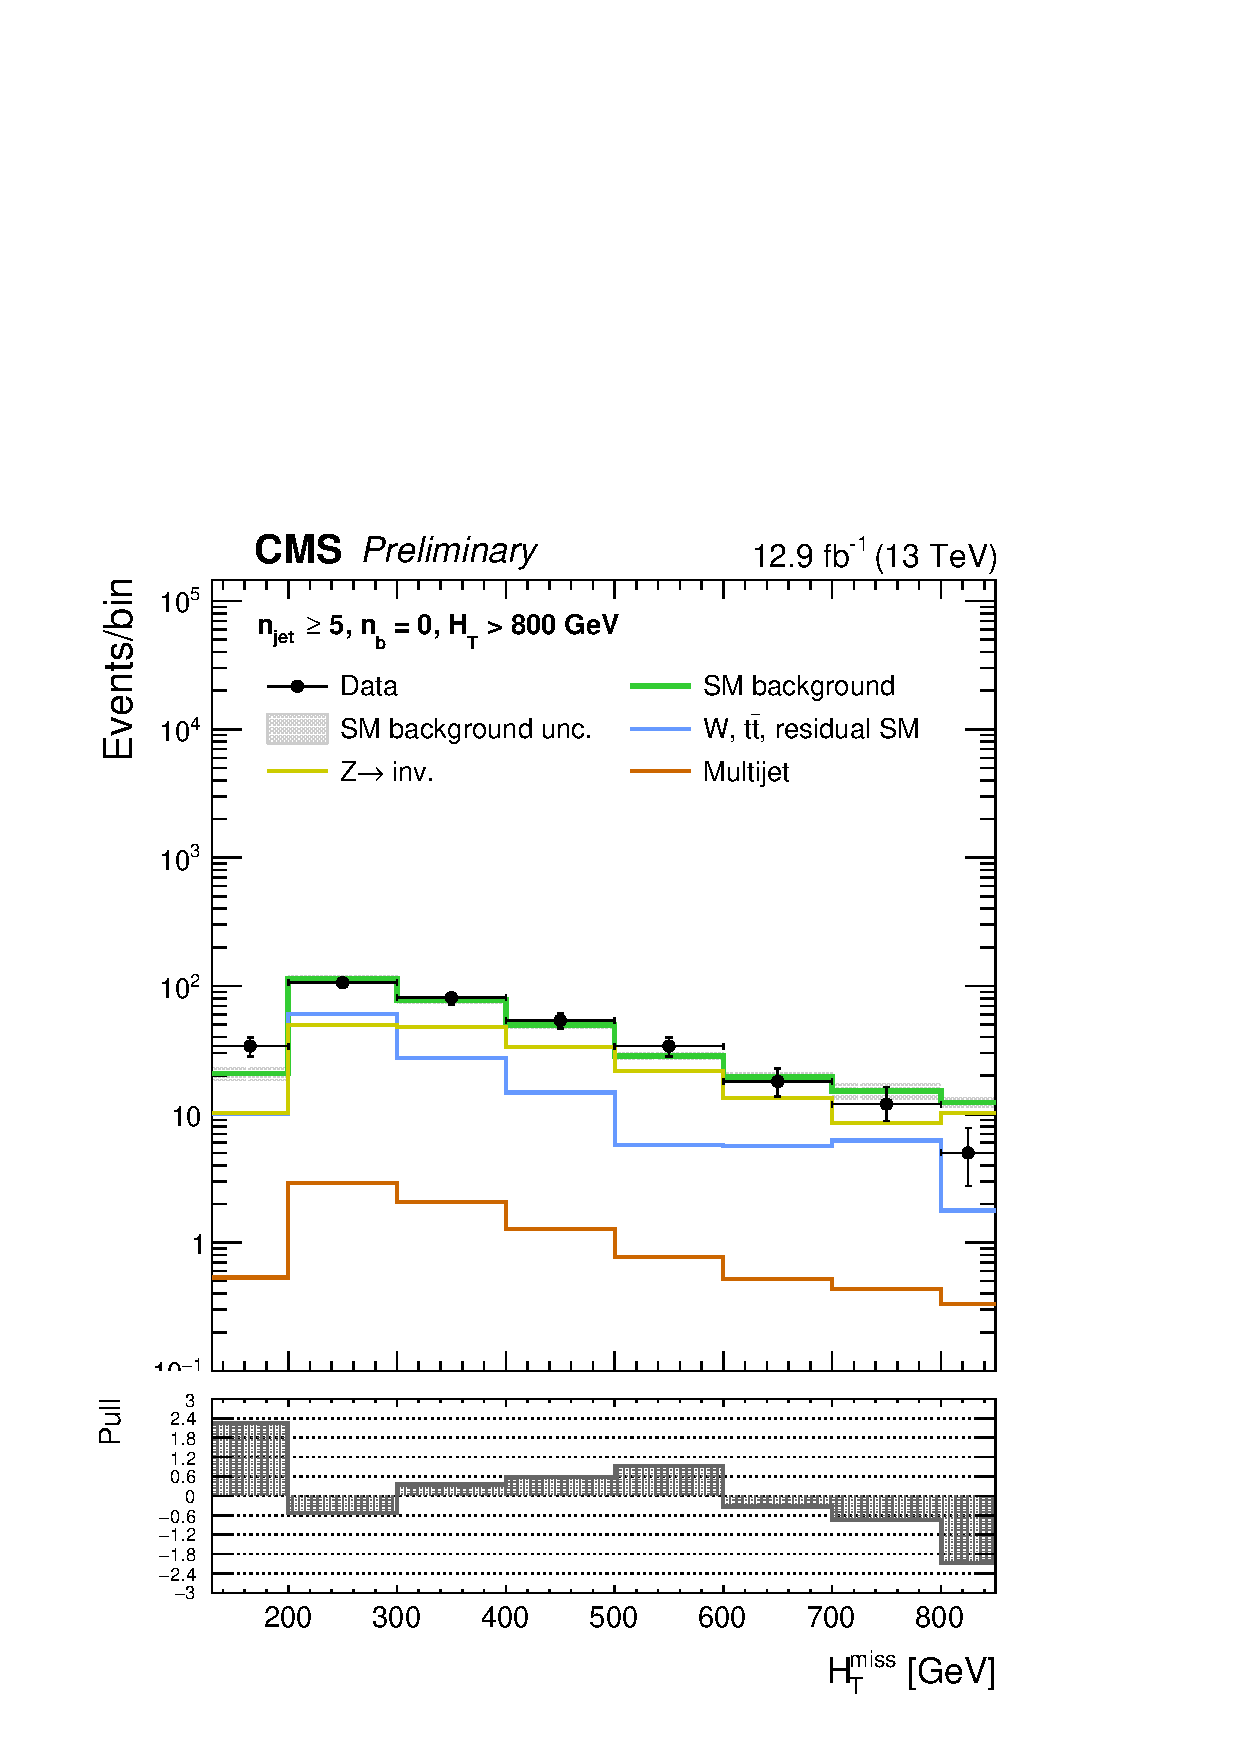
\includegraphics[width=0.49\textwidth]{figs/analysis/results/mhtShape_eq0b_ge5j_800_Inf_fit_b.pdf}
    }~~
  \subfloat[Symmetric topology, high \nj, \nb and \HT]{
    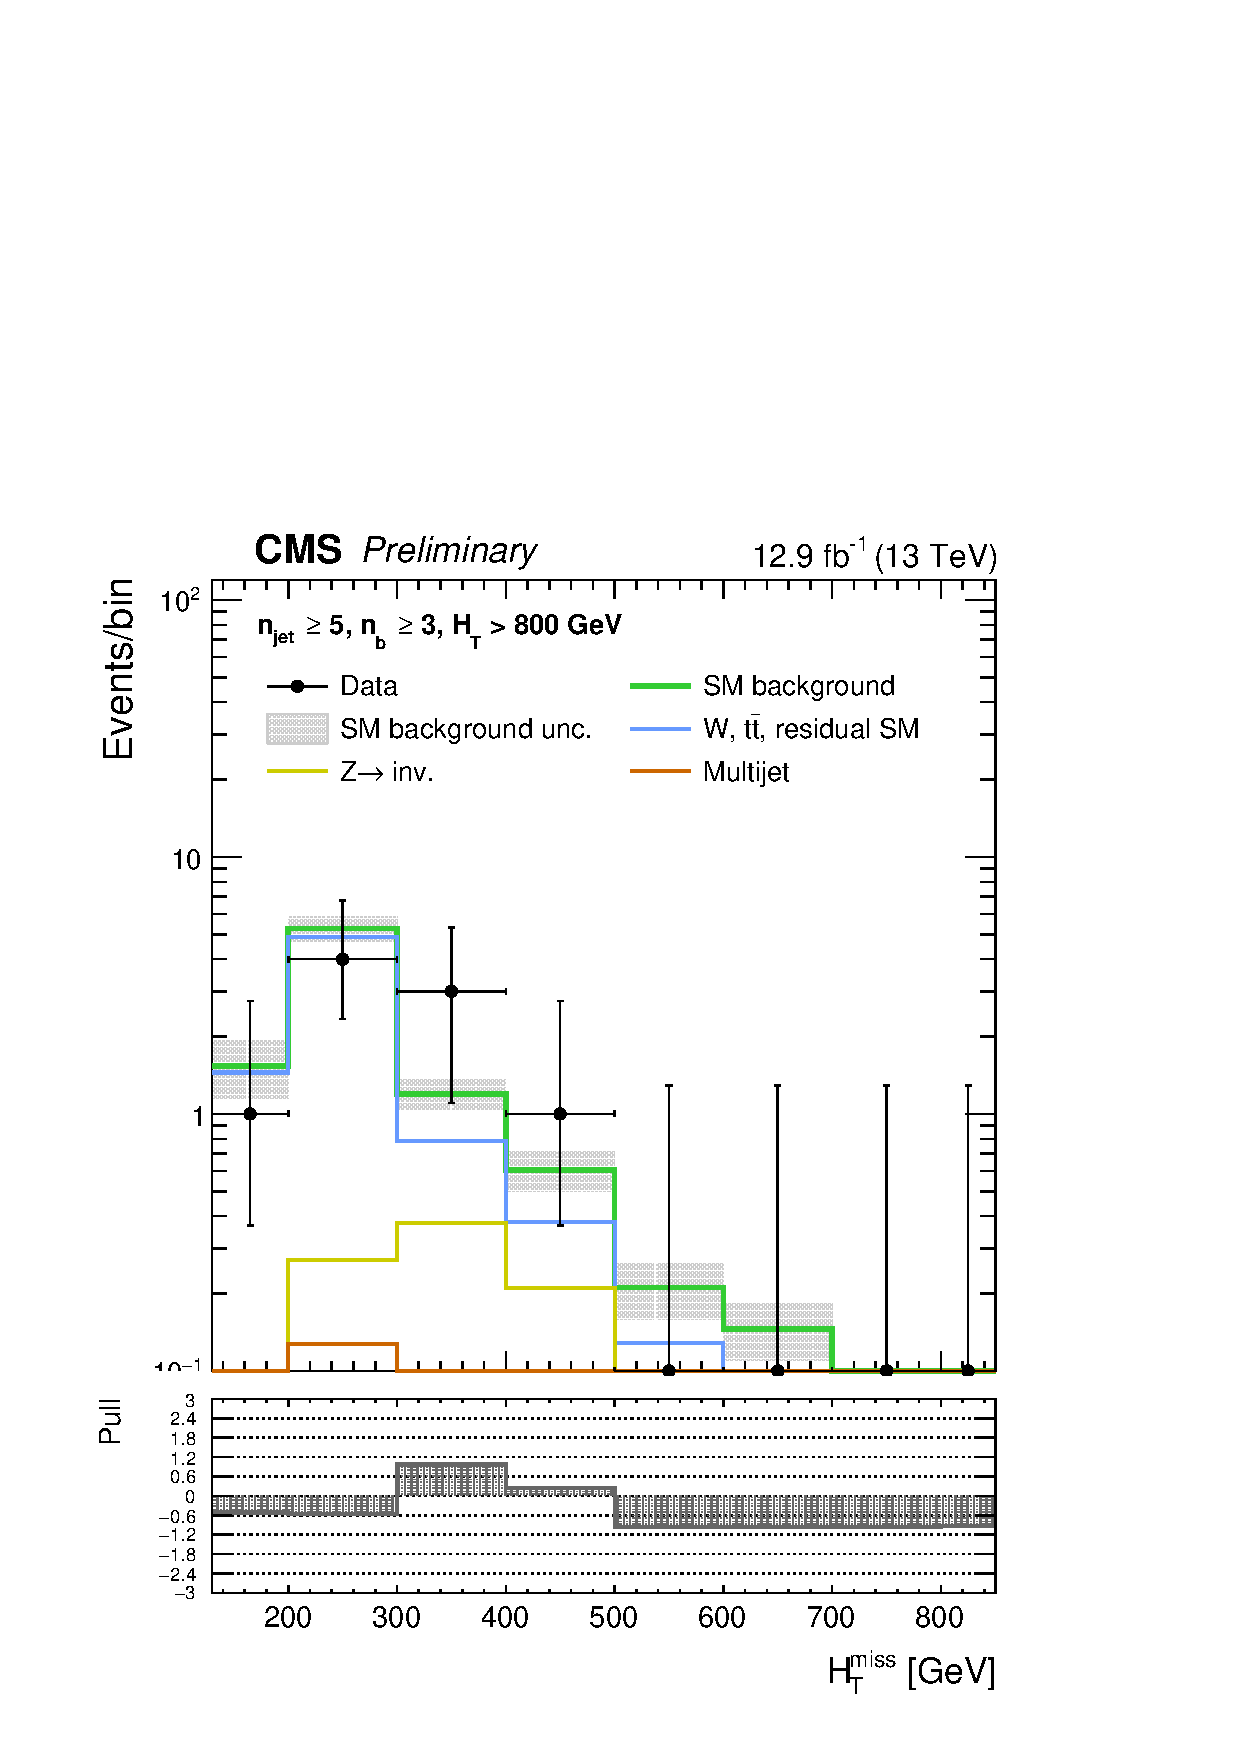
\includegraphics[width=0.49\textwidth]{figs/analysis/results/mhtShape_ge3b_ge5j_800_Inf_fit_b.pdf}
    }
  \end{center}
  \caption{The total event yields in data (solid black circles) and
  the \SM expectations with their associated uncertainties (green
  histogram with shaded band) as a function of \MHT for events in the
  signal region for four representative signal region categories. The
  final bin of each histogram is an overflow bin. Under this is the
  significance of deviations (pulls) observed in data with respect to
  the \SM expectations. \label{fig:mht-templates} 
  }
\end{figure*}

% some representative systematics or not...
\clearpage

%%%%%%%%%%%%%%%%%%%%
\section{Interpretation of the results}
\label{sec:signalModel}

As there is no excess observed in the data above that expected from
the \SM background prodiction, limits are set on the parameters of
possible \SUSY models. For the interpretation of the results, the
simplified models discussed in Sec.~\ref{sec:simplifiedModels} are
utilised. Four particular models are used to interpret the results of
the analysis. The models are named based on their production topology,
with gluino pair produced models being prefixed with \emph{T1} and
squark pair produced models being prefixed with \emph{T2}. Two
varieties of the gluino pair produced models are shown in
Fig.~\ref{fig:simplified-models-feyn-gluino}, in which the gluino
decays via third generation quarks. Their corresponding squark pair
produced models are shown in
Fig.~\ref{fig:simplified-models-feyn-3rdGen}.  
% Finally, models in
% which the gluinos or squarks decay to light quarks are considered and
% shown in Fig.~\ref{fig:simplified-models-feyn-light}.

The predicted yields for each of these signal models are taken
directly from \MC simulation. To be able to understand which mass
range of these models is excluded by the result, a large number of
different simulations are produced for a range of gluino, squark and
neutralino masses, $m_{\tilde{g}}$, $m_{\tilde{q}}$ and
$m_{\tilde{\chi^0_1}}$ respectively. For each of these mass points it
is considered whether the model is compatible with the observed
results or not. If it is not, it is deemed to be excluded to a
particular
degree of certainty.

\begin{figure}[h!]
  \begin{center}
    \subfloat[T1bbbb]{
      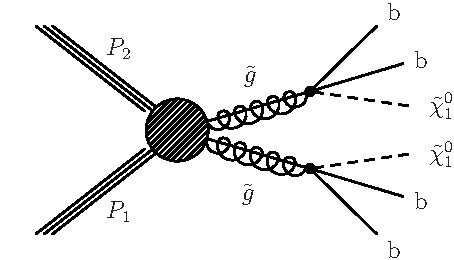
\includegraphics[width=0.3\textwidth]{figs/analysis/interpretation/T1bbbb_feyn}
      \label{fig:T1bbbb_feyn}
    } ~~
    \subfloat[T1tttt]{
      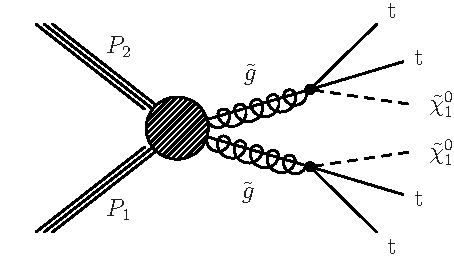
\includegraphics[width=0.3\textwidth]{figs/analysis/interpretation/T1tttt_feyn}
      \label{fig:T1tttt_feyn}
    } ~~
    \caption{
      Feynman diagram of simplified models in which gluinos are pair
      produced and decay to an \LSP via third generation squarks. 
    }
    \label{fig:simplified-models-feyn-gluino}
  \end{center}
\end{figure}

\begin{figure}[h!]
  \begin{center}
    \subfloat[T2tt]{
      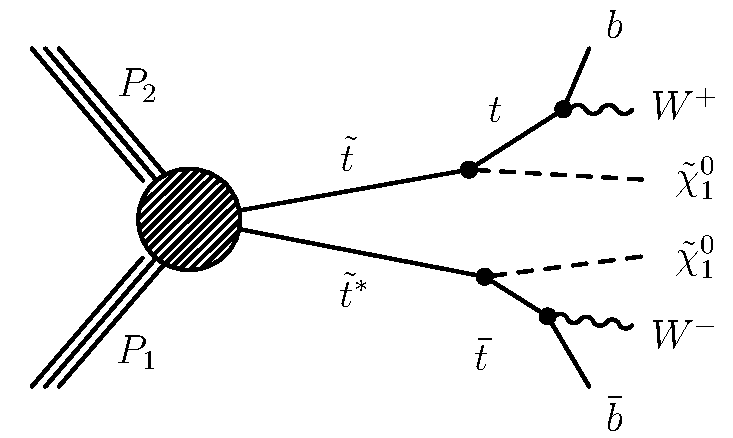
\includegraphics[width=0.3\textwidth]{figs/analysis/interpretation/T2tt_feyn}
      \label{fig:T2tt_feyn}
    } ~~
    \subfloat[T2bb]{
      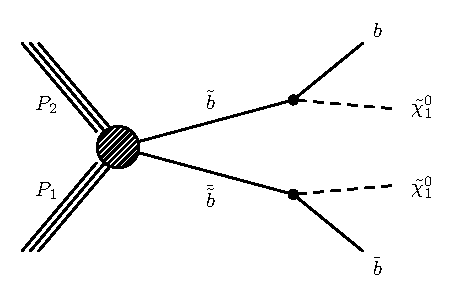
\includegraphics[width=0.3\textwidth]{figs/analysis/interpretation/T2bb_feyn}
      \label{fig:T2bb_feyn}
    }
    \caption{
      Feynman diagram of simplified models in which stops or sbottoms are pair
      produced and decay to an \LSP via third generation squarks. 
    }
    \label{fig:simplified-models-feyn-3rdGen}
  \end{center}
\end{figure}

% \begin{figure}[h!]
%   \begin{center}
%     \subfloat[T1qqqq]{
%       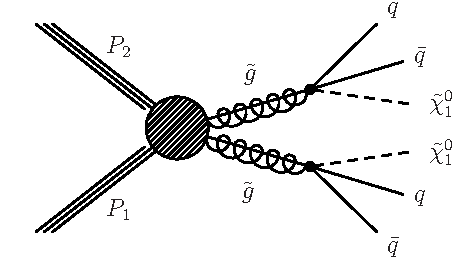
\includegraphics[width=0.3\textwidth]{figs/analysis/interpretation/T1qqqq_feyn}
%       \label{fig:T1qqqq_feyn}
%     } ~~
%     \subfloat[T2qq]{
%       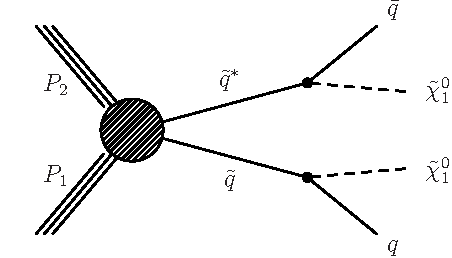
\includegraphics[width=0.3\textwidth]{figs/analysis/interpretation/T2qq_feyn}
%       \label{fig:T2qq_feyn}
%     }
%     \caption{
%       Graphical representation of the production and decay of supersymmetric particles 
%       in ``light-flavour models'', i.e. with gluinos/squarks decaying to light quarks. 
%     }
%     \label{fig:simplified-models-feyn-light}
%   \end{center}
% \end{figure}

\subsection{Uncertainties on signal models}

Sources of systematic uncertainty are propagated to the predicted
yields from the \MC simulation of the signal models. These
uncertainties are considered across all the (\HT,\nj,\nb) categories,
as well as the \MHT shapes. Most of the uncertainties are considered
in the same way as those in the \SM background prediction,
Sec.~\ref{sec:simUnc}. Due to the fact that the signal model yields come from
simulation, an additional uncertainty on the total integrated
luminosity is included. Additionally, an extra correction factor is
applied to the number of jets from initial state radiation. This also
has an associated uncertainty. Each of these uncertainties must be
determined for each independent simplified model. A summary of the
uncertainties for a representative T2bb simplified model and their
correlation across all categories is shown in
Tab.~\ref{tab:signal_systs}. The \emph{normalisation} uncertainties
just effect the total yield in each (\HT,\nj,\nb), while the
\emph{shape} uncertainties include variations in the \MHT shape.  

\begin{table}[h!]
  \caption{ The magnitude of uncertainties in the signal model yields
  in the case of a T2bb simplified model.
    }  
  \label{tab:signal_systs}
  \centering
  \footnotesize
  \begin{tabular}{ lccc }
    \hline
    Systematic source\T\B          & Type          & Correlated & Typical magnitude (\%) \\
    \hline
    Luminosity\T                   & Normalisation & Yes        & 6.2                    \\
    Monte Carlo statistics         & Norm. + shape & No         & 1--50                  \\
    Jet energy scale               & Norm. + shape & Yes        & 3--10                  \\
    b-tag efficiency scale factors & Norm. + shape & Yes        & 5--40                  \\
    Lepton scale factors           & Normalisation & Yes        & 1--5                   \\
    Pile-up                        & Norm. + shape & Yes        & 0--5                   \\
    Trigger efficiency             & Norm. + shape & Yes        & 0--4                   \\
    Initial state radiation        & Norm. + shape & Yes        & 1--20                  \\
    Modelling of \MHT         & Normalisation & Yes        & 1--5                   \\
%    Renormalisation/factorisation & Norm. + shape & No         & 10                     \\
    \hline
  \end{tabular}
\end{table}

% \begin{itemize}
%   \item Luminosity: 6.2 \%, taken as correlated across all bins.
%   \item Trigger: systematic measured using the difference between the
%   electron and muon reference triggers (see Sec.~\ref{sec:triggers}).
%   \item MC statistics:  uncorrelated bin-by-bin uncertainty, affecting
%   the shape of the signal.  \item Pileup reweighting: 5\% uncertainty
%   on the minimum bias cross section (see
%   Sec.~\ref{sec:pileup-reweighting}).  \item b-tag efficiency:
%   uncertainties on the FullSim and FastSim b-tag scale factors are
%   propagated and taken as correlated across the bins. These are
%   uncorrelated for mis-tag and efficiency systematics.  \item Lepton
%   efficiency: uncertainty on the lepton scale factors is propagated
%   and taken as correlated across the bins.  \item Jet energy scale:
%   uncertainty on the jet energy corrections is propagated and taken as
%   correlated across the bins.  \item Initial State Radiation (ISR): A
%   systematic of half the correction factor applied to the MC per
%   number of ISR jets is taken as correlated across the bins.
% \end{itemize}

\subsection{Exclusion limits}

For each of the mass points and all the simplified models introduced
in Sec.~\ref{sec:signalModel}, an upper limit at a 95\% \CL on the
cross section to produce the pair of sparticles considered in the
model is determined. This limit is produced under a background plus
signal hypothesis with a modified frequentist approach. The potential
contribution of the simplified models to each of the analysis bins in
the signal region is considered. The statistical approach uses a
one-sided profile likelihood ratio as the test statistic. The limit is
set using the \emph{CL$_S$} criterion ~\cite{junk, read} and the
asymptotic formulae~\cite{Cowan:2010js} are used to approximate the
distributions of the test statistics under the relevant hypothesis
(either background only or signal plus background). 

The results of the exclusion of two gluino models (T1tttt and T1bbbb)
and two squark models (T2tt and T2tt) are shown in
Fig.~\ref{sec:signalModel}. The 95\% \CL upper limit on the cross
section is plotted as a two dimensional histogram with a colour scale
for a range of different sparticle and \LSP masses. The theoretical
cross sections of the models are determined with \NLO
accuracy and there is an assumption of a 100\% branching ratio to
final state of each model. Based on this, observed (black) and
expected (red) exclusion contours are plotted with their $\pm1\sigma$
uncertainty bands, encapsulating the experimental uncertainty for the
limit and the theoretical uncertainties of the signal model cross
section. For the T2tt model, the low mass region is blanked out when
the mass of the stop, $m_{\tilde{t}}$, is close to the mass of the top
quark and the total \MET in the event is small. This is due to issues
in the \MET reconstruction of the simulated \SUSY model events in this
region of parameter space.

In gluino mediated models, the gluino mass is excluded up to 
$1775~\gev$ and the \LSP, $\tilde{\chi}^0$, up to $1175~\gev$. In the
squark mediated models, the sbottom mass is excluded up to $1025~\gev$
and the stop mass is excluded up to $875~\gev$ with \LSP exclusions of
$525~\gev$ and $350~\gev$ respectively. The strongest observed
exclusions are summarised in Tab.~\ref{tab:simplified-models-limits}.
This presents a significant improvement on some of the limits found
with the $19.5~\ifb$ result made with $\sqrt{s}=8~\tev$ proton
collisions from Run~1. In the best cases the gluino masses were
excluded at $<1400~\gev$ and the sbottom masses to $<800~\gev$
\cite{smsTwiki}.

\begin{figure}[h!]
  \begin{center}
    \subfloat[T2tt: Upper limit on the cross section in the
    $(m_{\mathrm{stop}},m_{\mathrm{\LSP}})$ plane]{
      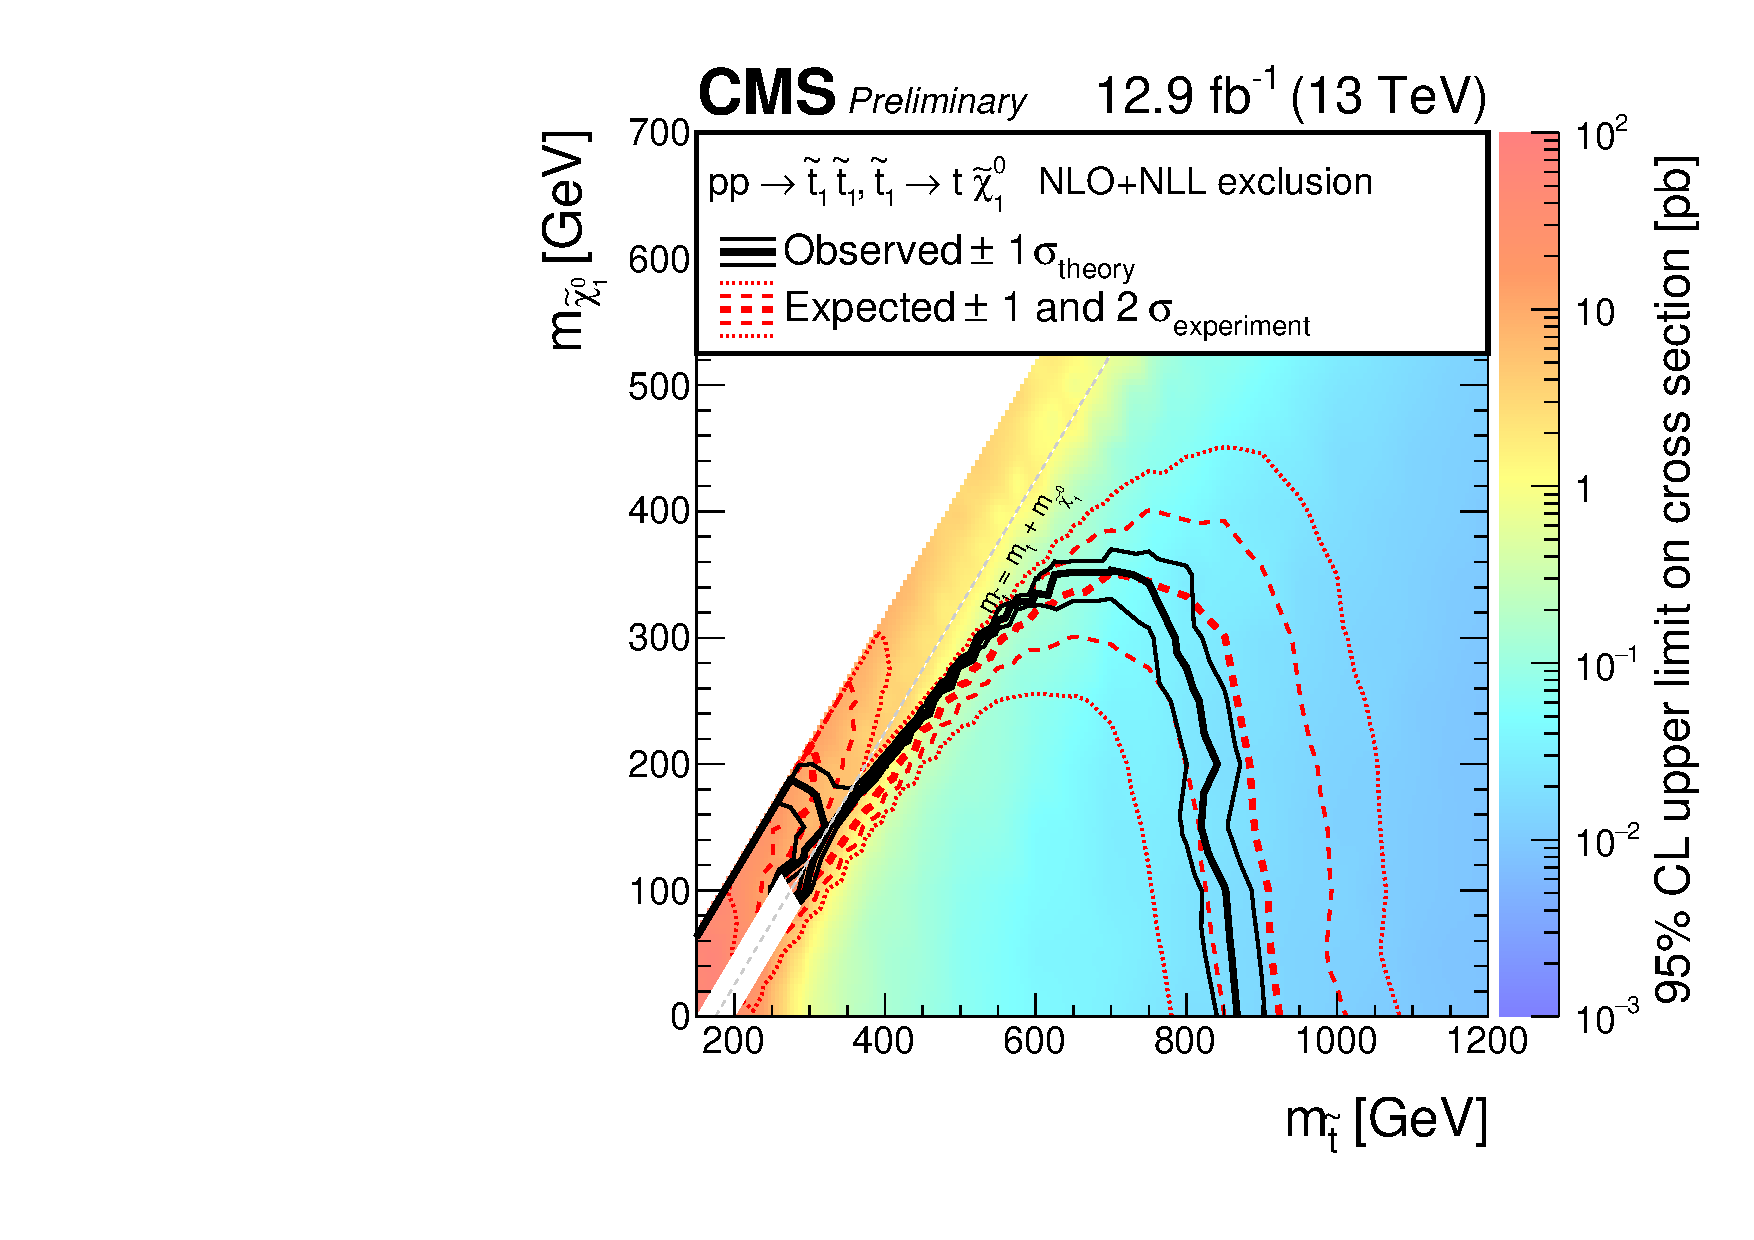
\includegraphics[width=0.5\textwidth]{figs/analysis/interpretation/T2ttXSEC}
      \label{fig:T2tt_excl}
    } ~~
    % \subfloat[T2tt: $\epsilon_{sig}^{\mathrm{4\,cat}}$]{
    %   \includegraphics[width=0.45\textwidth]{figures/jetRanking/T2tt/eff/T2tt_merging_4_cats}
    %   \label{fig:T2tt_eff}
    % } ~~
    % \subfloat[T2tt: $\epsilon_{sig}^{\mathrm{4\,cat}}/\epsilon_{sig}^{\mathrm{tot}}$]{
    %   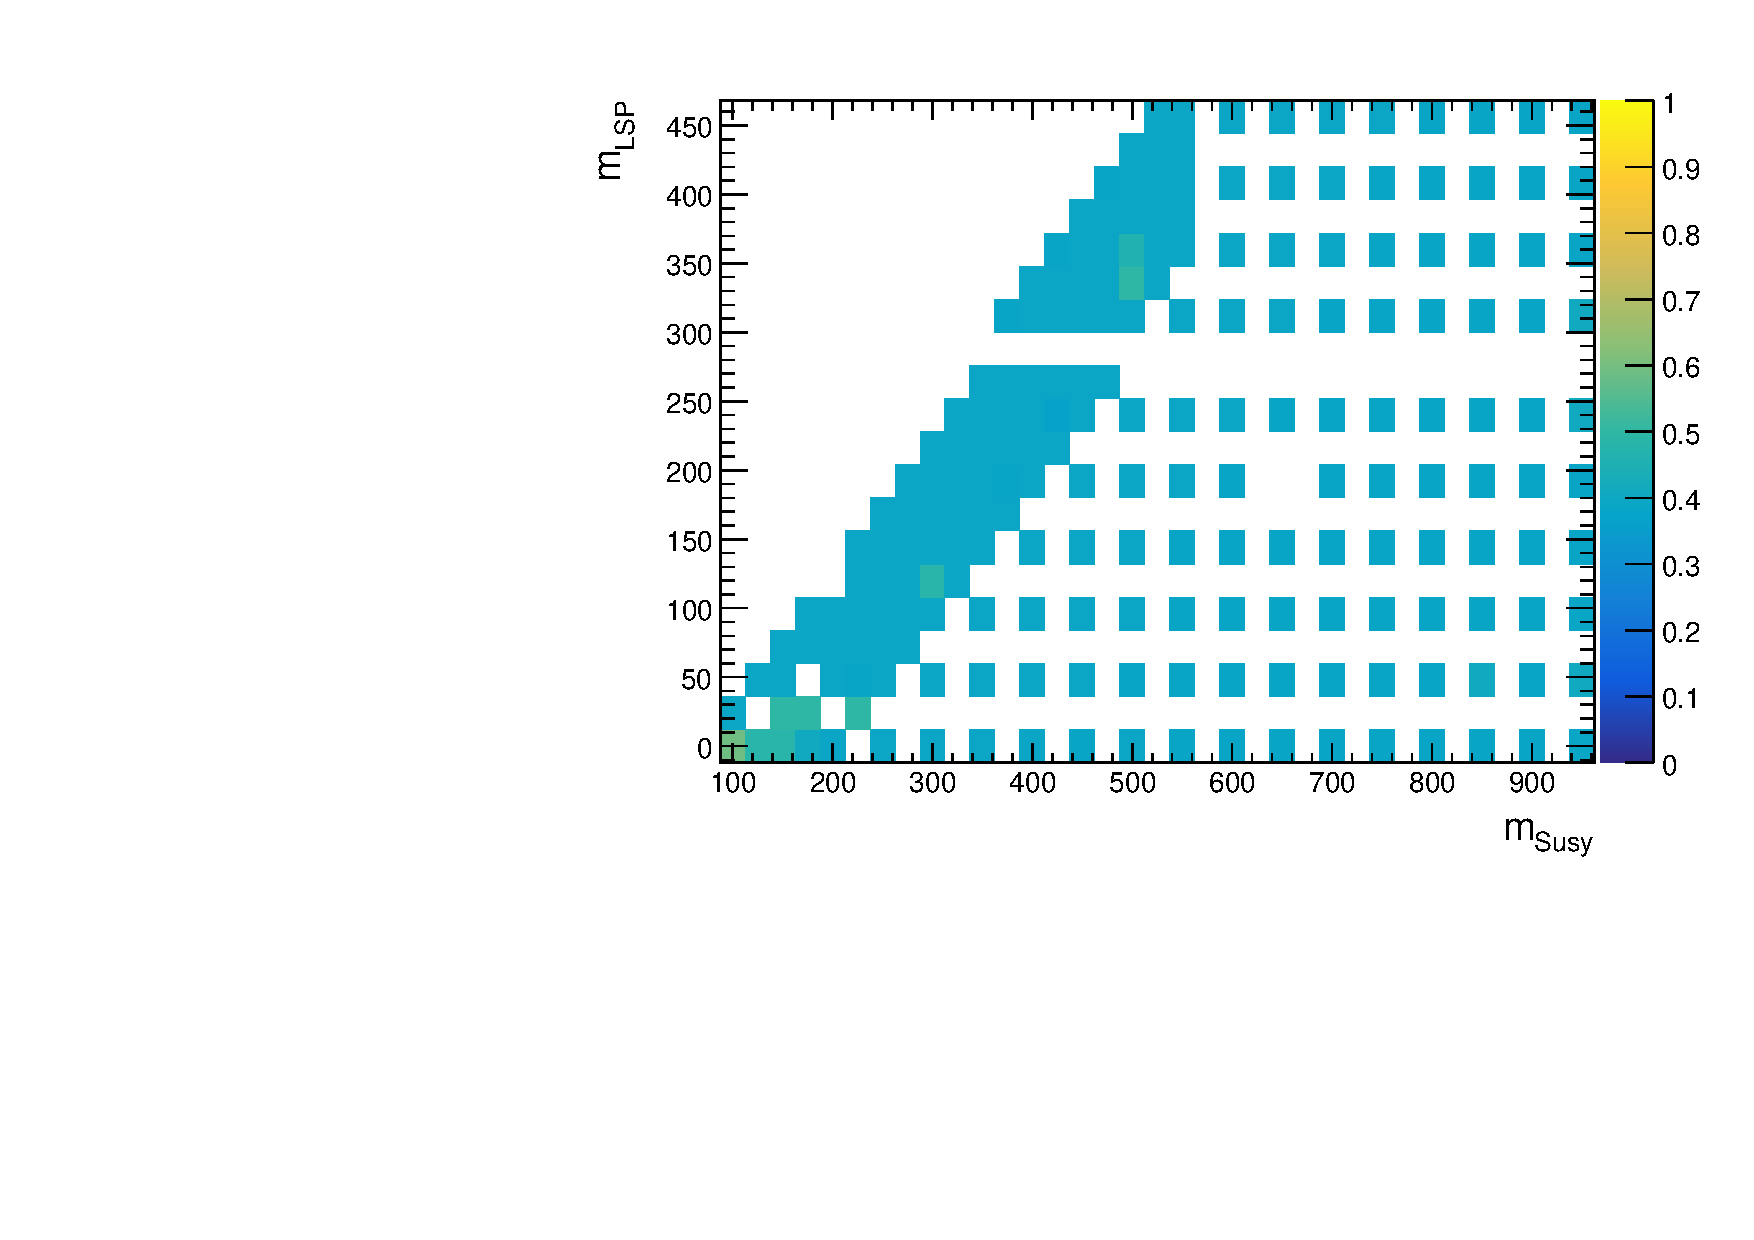
\includegraphics[width=0.45\textwidth]{figures/susyResults/T2tt_doubleRatioAcceptance}
    %   \label{fig:T2tt_eff_doubleRatio}
    % }
    \label{fig:T2tt}
    \subfloat[T2bb: Upper limit on the cross section in the
    $(m_{\mathrm{sbottom}},m_{\mathrm{\LSP}})$ plane]{
      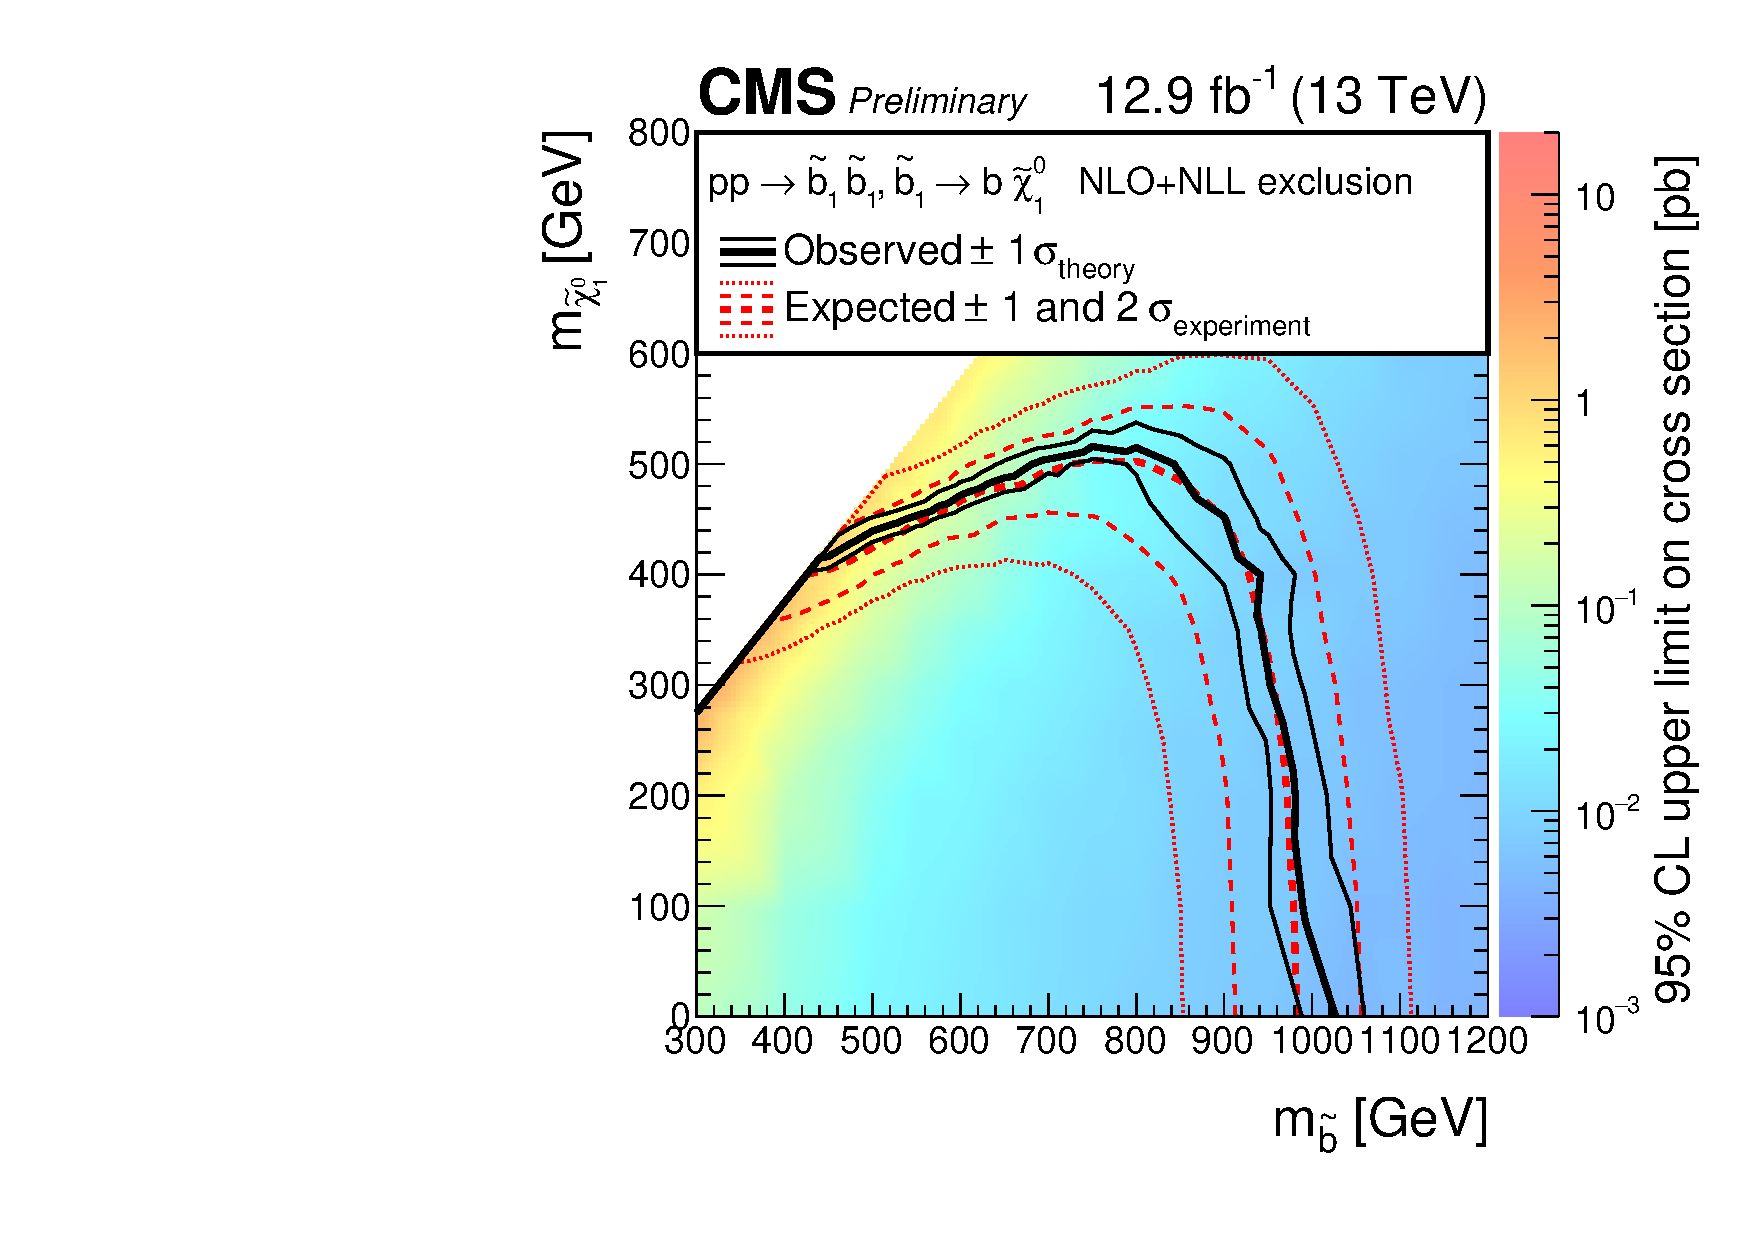
\includegraphics[width=0.5\textwidth]{figs/analysis/interpretation/T2bbXSEC}
      \label{fig:T2bb_excl}
    } \\
    % \subfloat[T2bb: $\epsilon_{sig}^{\mathrm{4\,cat}}$]{
    %   \includegraphics[width=0.45\textwidth]{figures/jetRanking/T2bb/eff/T2bb_merging_4_cats}
    %   \label{fig:T2bb_eff}
    % } ~~
    % \subfloat[T2bb: $\epsilon_{sig}^{\mathrm{4\,cat}}/\epsilon_{sig}^{\mathrm{tot}}$]{
    %   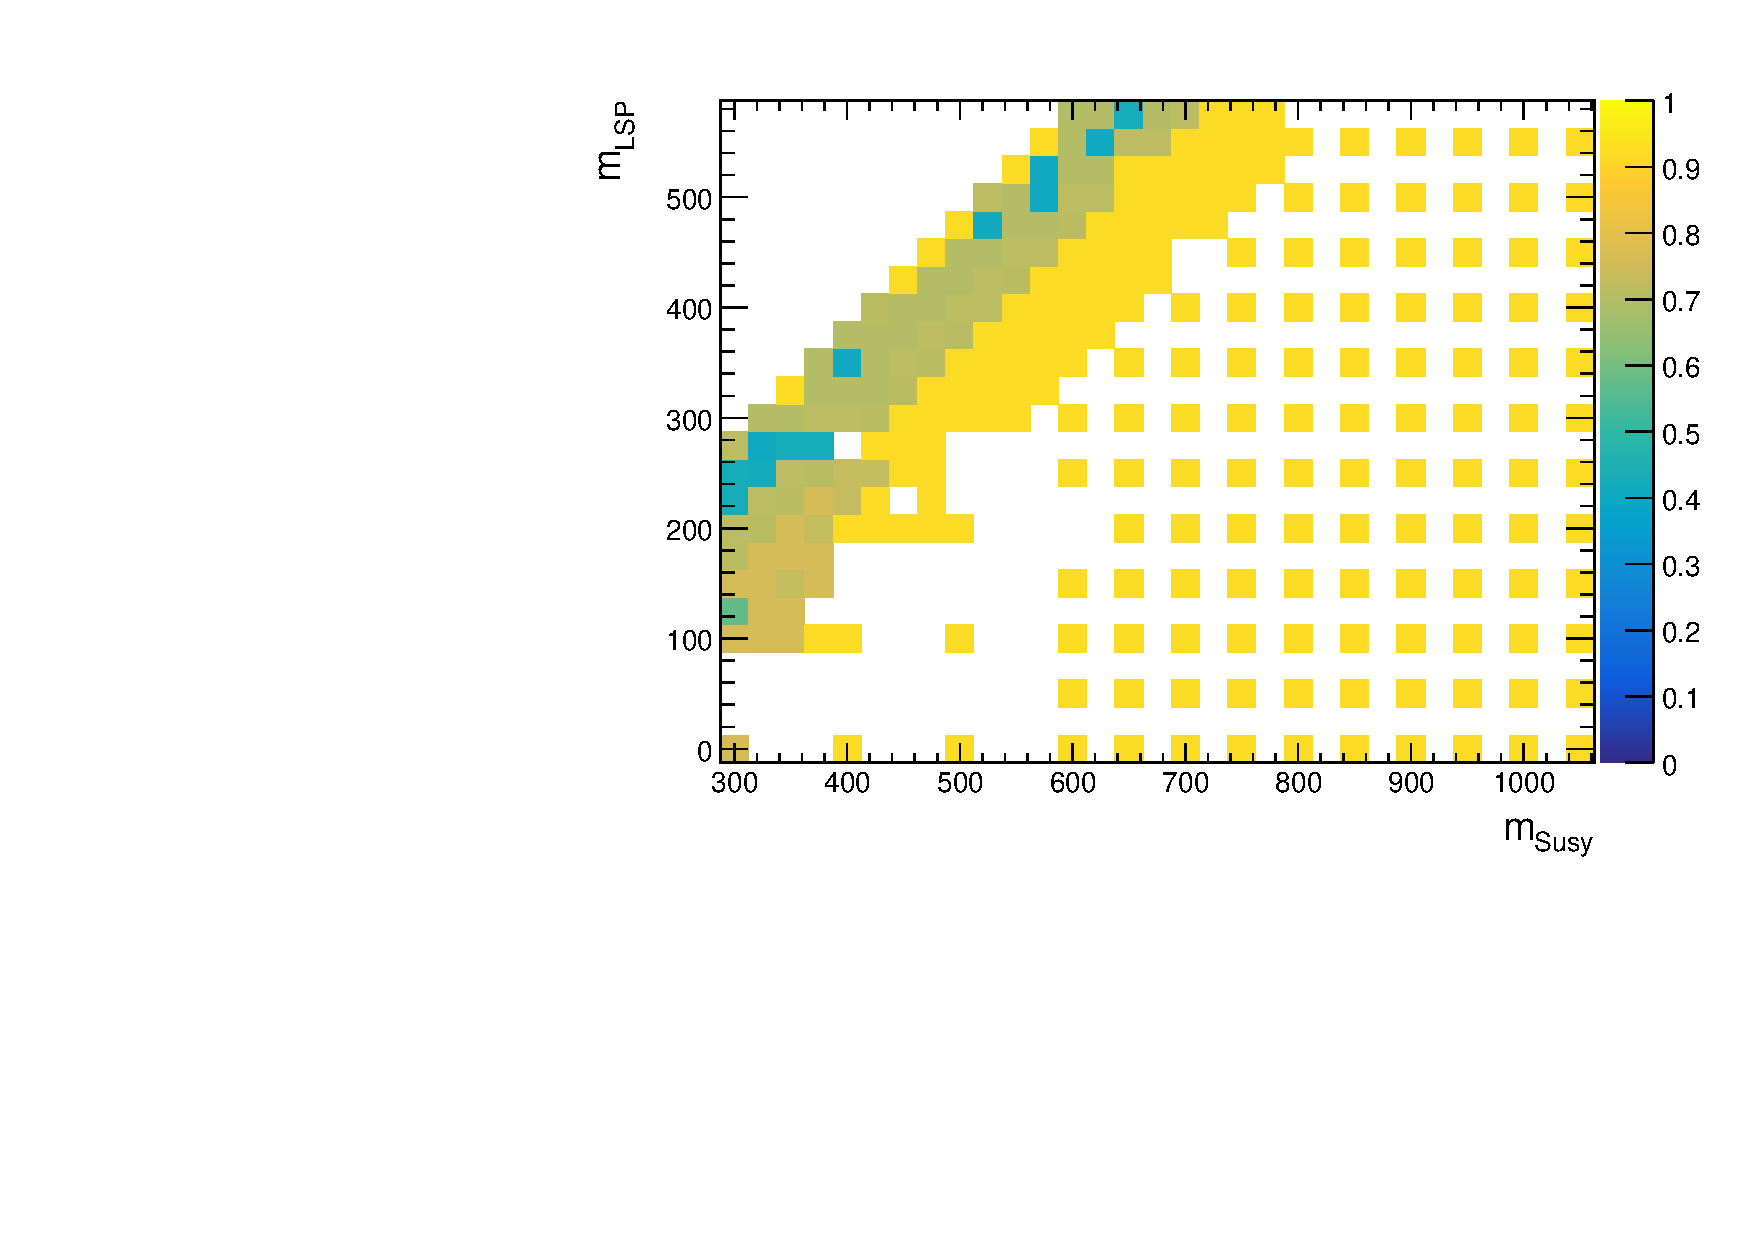
\includegraphics[width=0.45\textwidth]{figures/susyResults/T2bb_doubleRatioAcceptance}
    %   \label{fig:T2bb_eff_doubleRatio}
    % }
    
    \label{fig:T2bb}
    \subfloat[T1bbbb: Upper limit on the cross section in the
    $(m_{\mathrm{Gluino}},m_{\mathrm{\LSP}})$ plane]{
      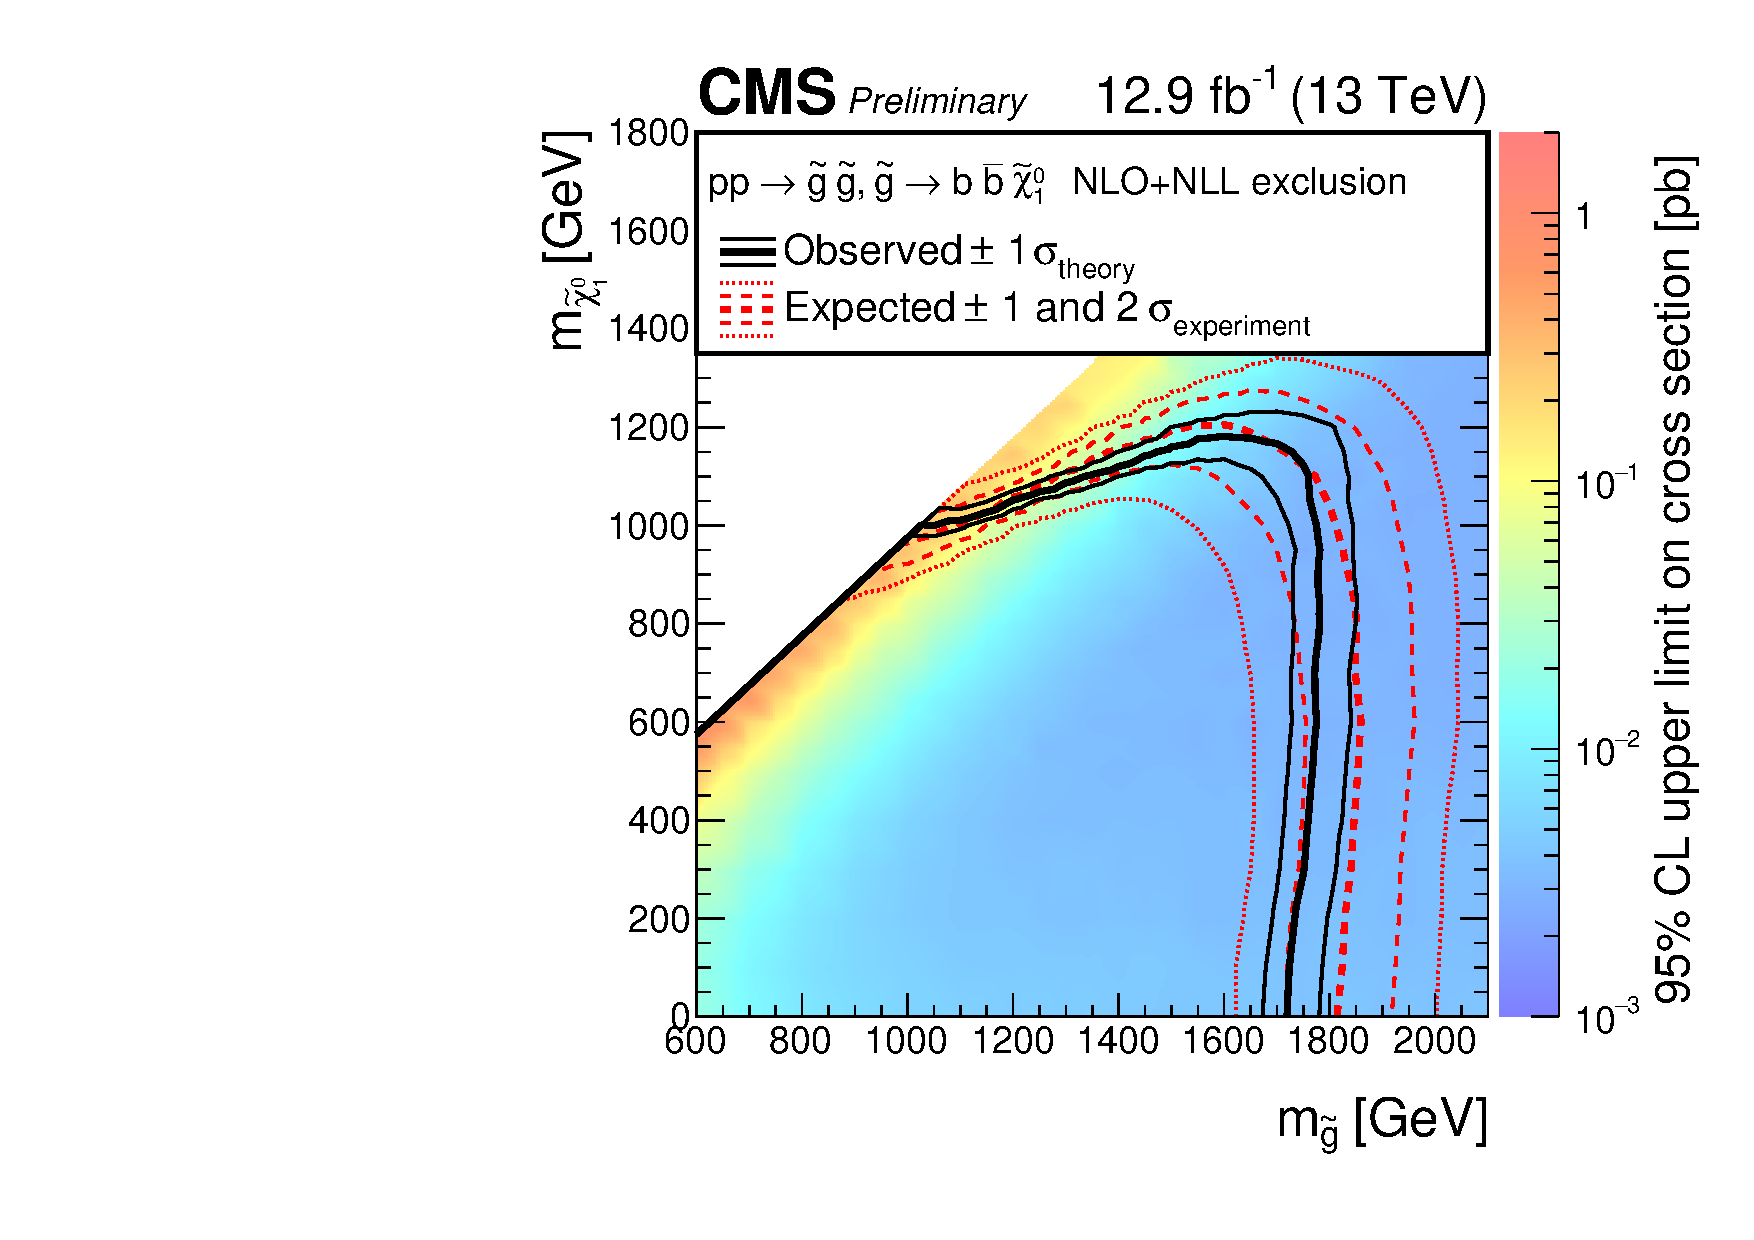
\includegraphics[width=0.5\textwidth]{figs/analysis/interpretation/T1bbbbXSEC}
      \label{fig:T1bbbb_excl}
    } ~~
    % \subfloat[T1bbbb: $\epsilon_{sig}^{\mathrm{4\,cat}}$]{
    %   \includegraphics[width=0.45\textwidth]{figures/jetRanking/T1bbbb/eff/T1bbbb_merging_4_cats}
    %   \label{fig:T1bbbb_eff}
    % } ~~
    % \subfloat[T1bbbb: $\epsilon_{sig}^{\mathrm{4\,cat}}/\epsilon_{sig}^{\mathrm{tot}}$]{
    %   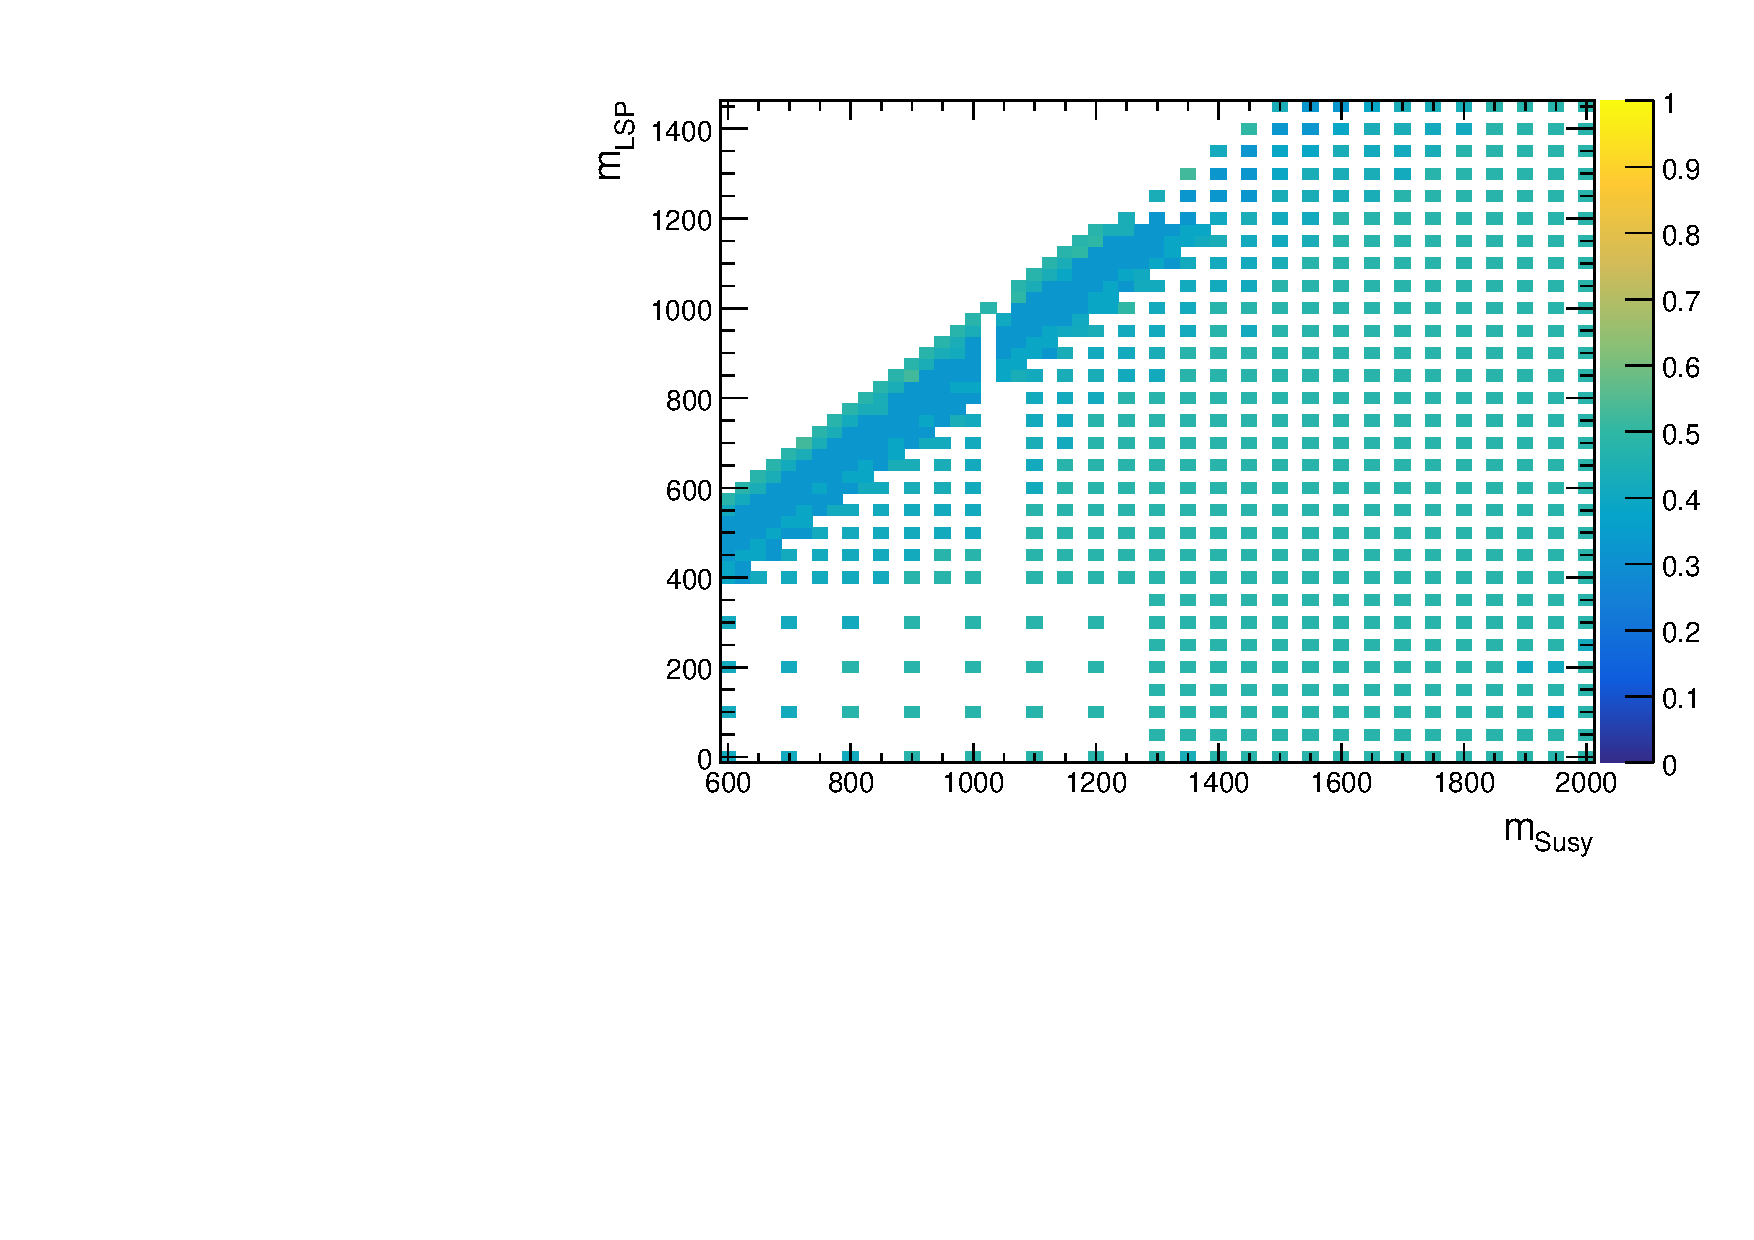
\includegraphics[width=0.45\textwidth]{figures/susyResults/T1bbbb_doubleRatioAcceptance}
    %   \label{fig:T1bbbb_eff_doubleRatio}
    % }
    \label{fig:T1bbbb}
    \subfloat[T1tttt: Upper limit on the cross section in the
    $(m_{\mathrm{Gluino}},m_{\mathrm{\LSP}})$ plane]{
      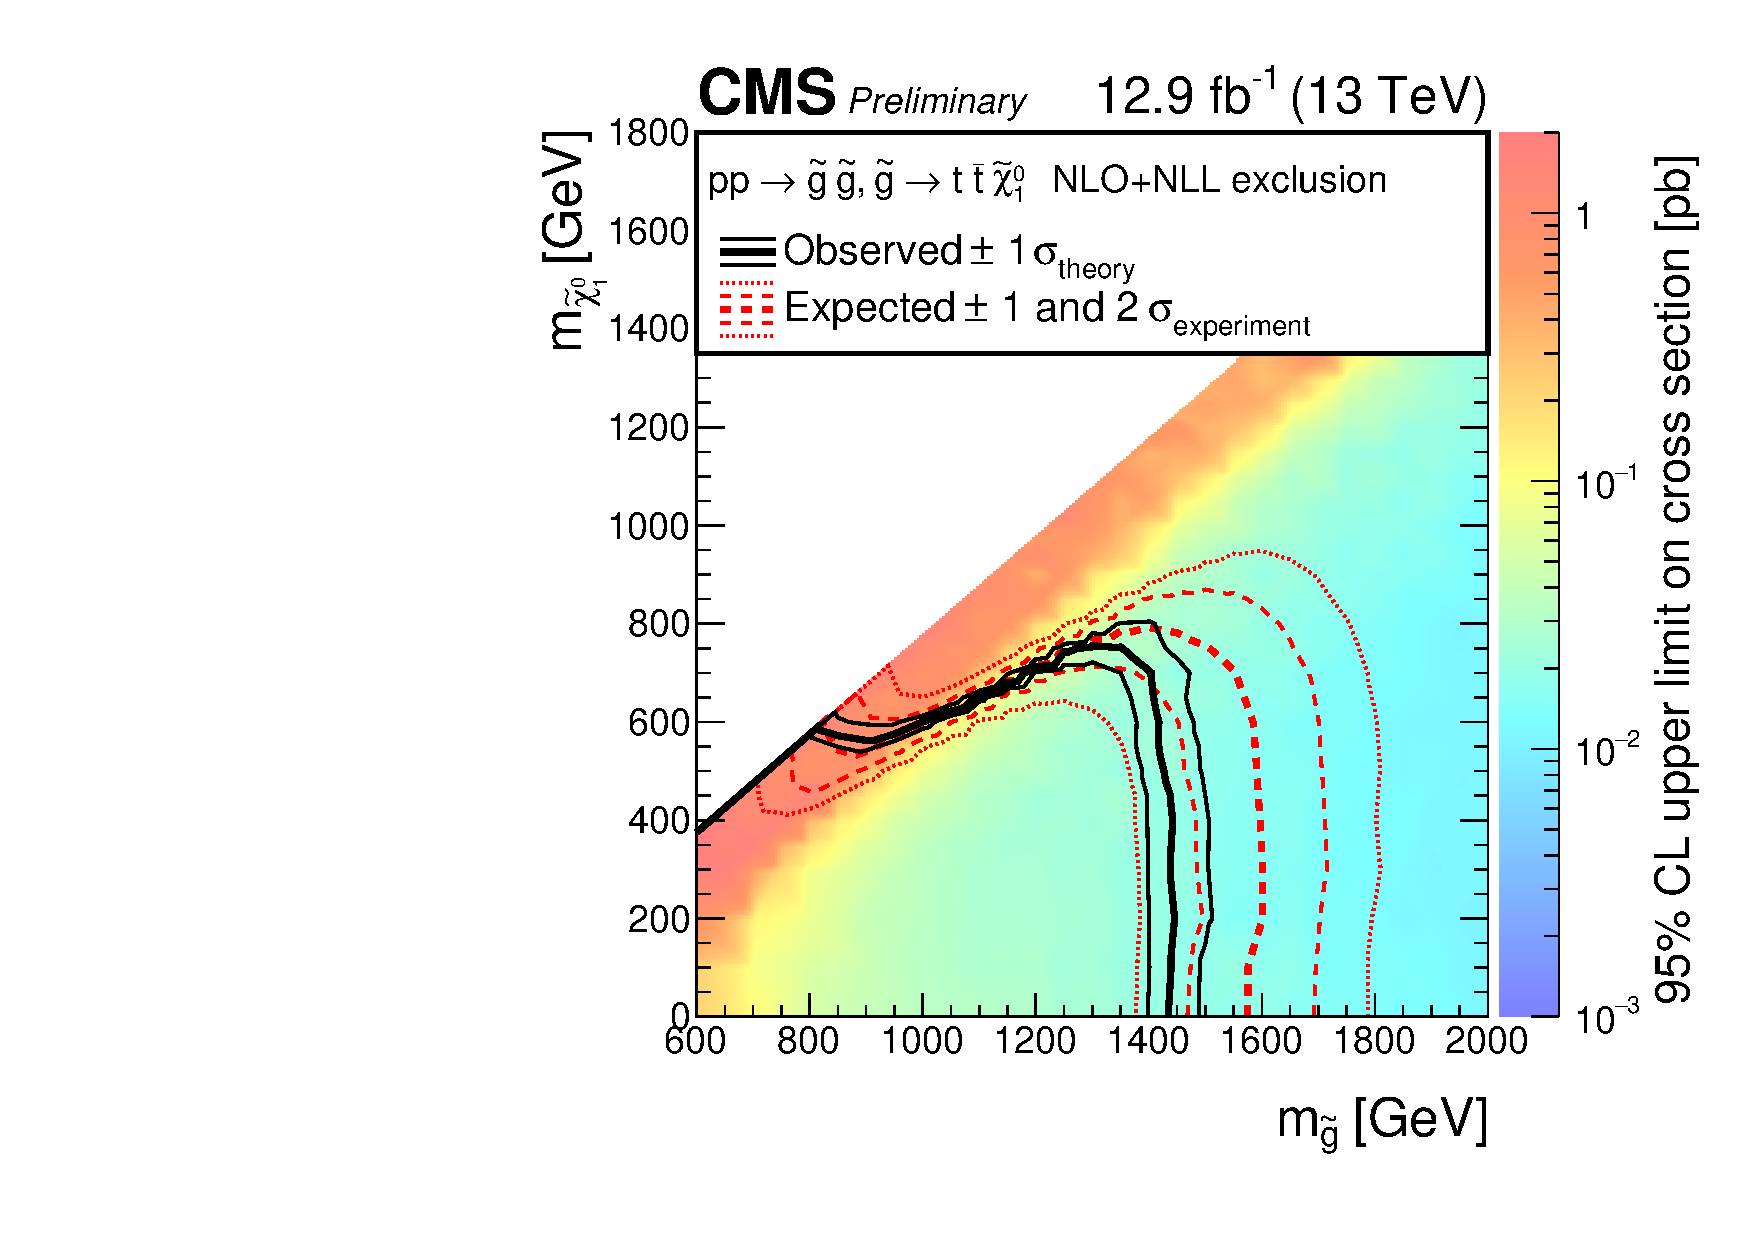
\includegraphics[width=0.5\textwidth]{figs/analysis/interpretation/T1ttttXSEC}
      \label{fig:T1tttt_excl}
    } \\
    % \subfloat[T1tttt: $\epsilon_{sig}^{\mathrm{4\,cat}}$]{
    %   \includegraphics[width=0.45\textwidth]{figures/jetRanking/T1tttt/eff/T1tttt_merging_4_cats}
    %   \label{fig:T1tttt_eff}
    % } ~~
    % \subfloat[T1tttt: $\epsilon_{sig}^{\mathrm{4\,cat}}/\epsilon_{sig}^{\mathrm{tot}}$]{
    %   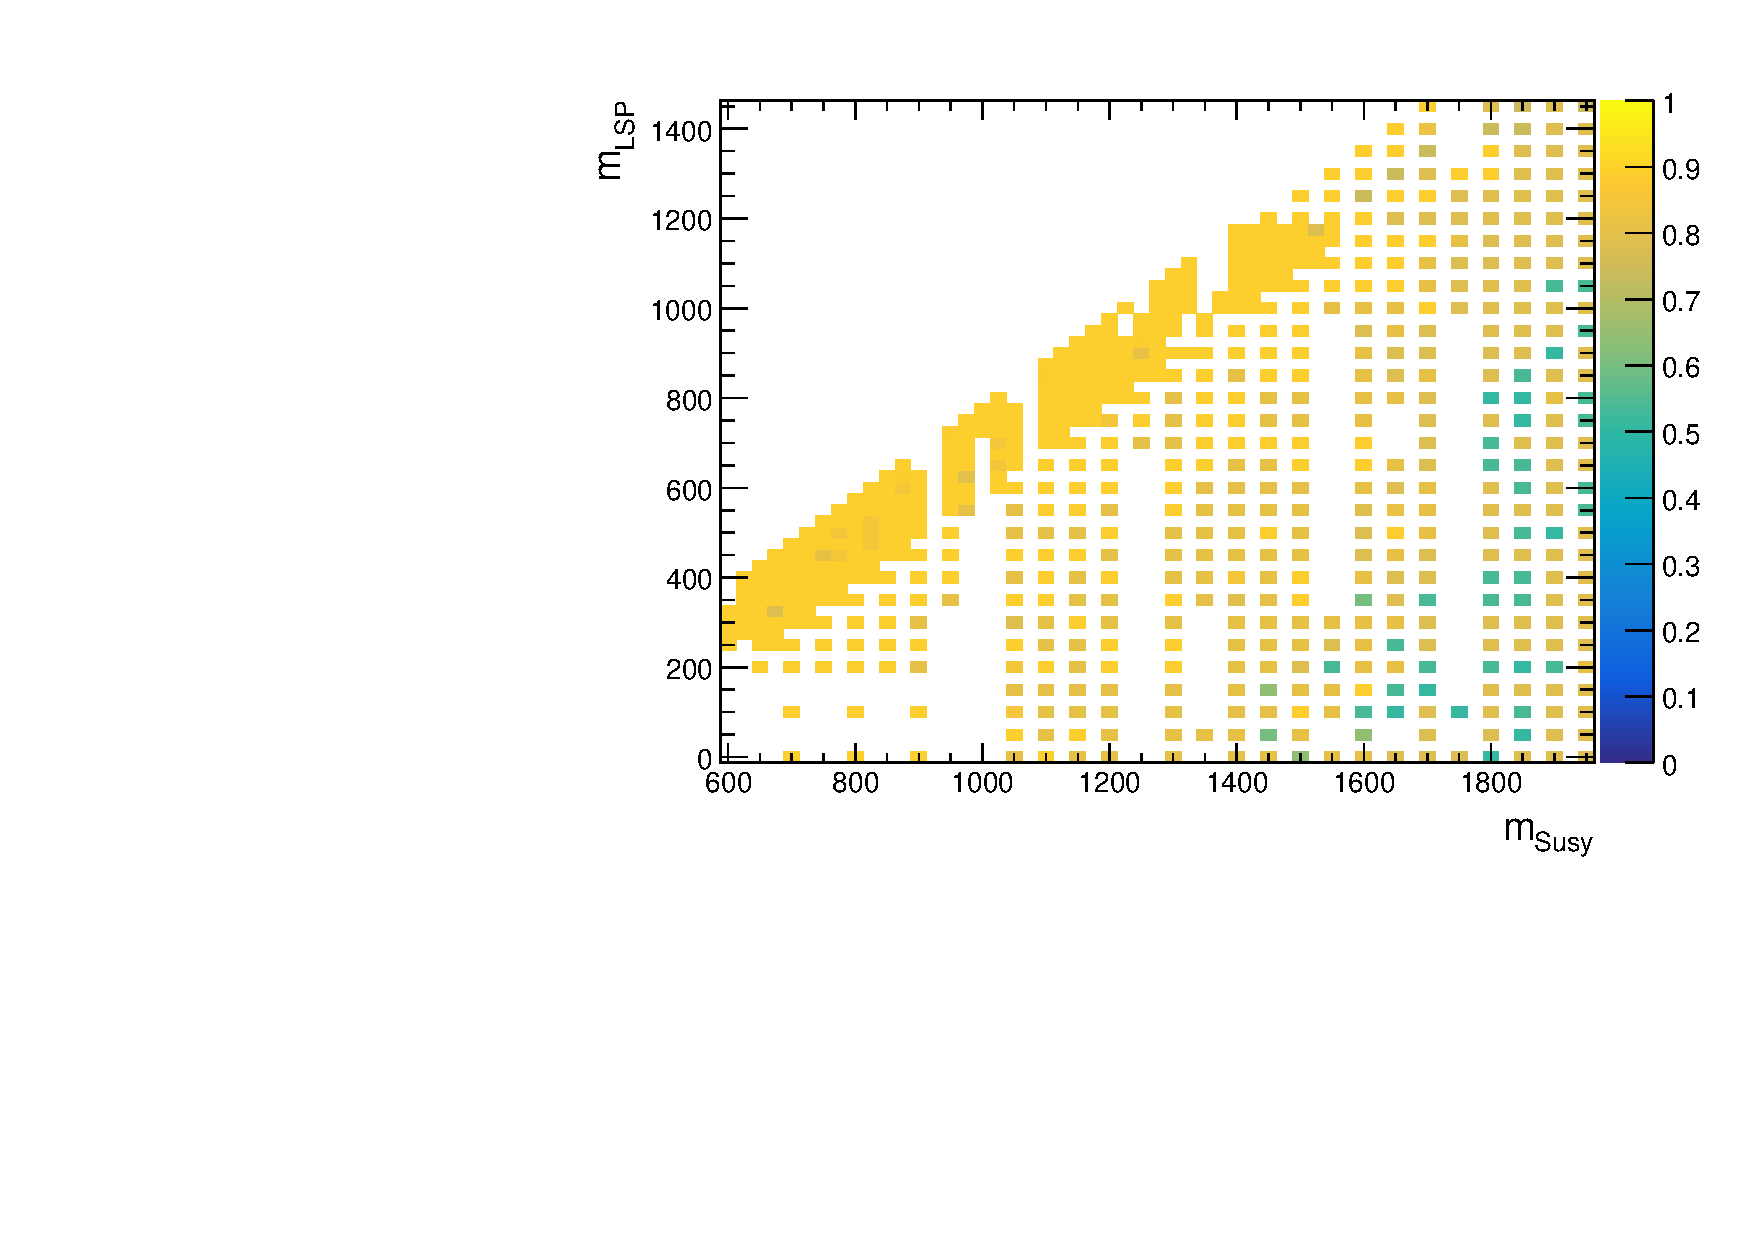
\includegraphics[width=0.45\textwidth]{figures/susyResults/T1tttt_doubleRatioAcceptance}
    %   \label{fig:T1tttt_eff_doubleRatio}
    % }
    \caption{
      The 95\% observed upper limit on the cross section (histogram),
      with the expected (dotted red line) and observed (black line)
      exclusion contours. Shown for a selection of \SUSY models discussed in
      Sec.~\ref{sec:signalModel}.
      % Bottom left: signal acceptance including the 4 most excluding jet categories. 
      % Bottom right: ratio of the signal acceptance including 4 categories to the acceptance including the whole signal region. 
    }
    \label{fig:T1tttt}
  \end{center}
\end{figure}


% \begin{figure}[h!]
%   \begin{center}
%     \subfloat[T2qq: Upper limit on the cross section in the
%     $(m_{\mathrm{squark}},m_{\mathrm{\LSP}})$ plane]{
%       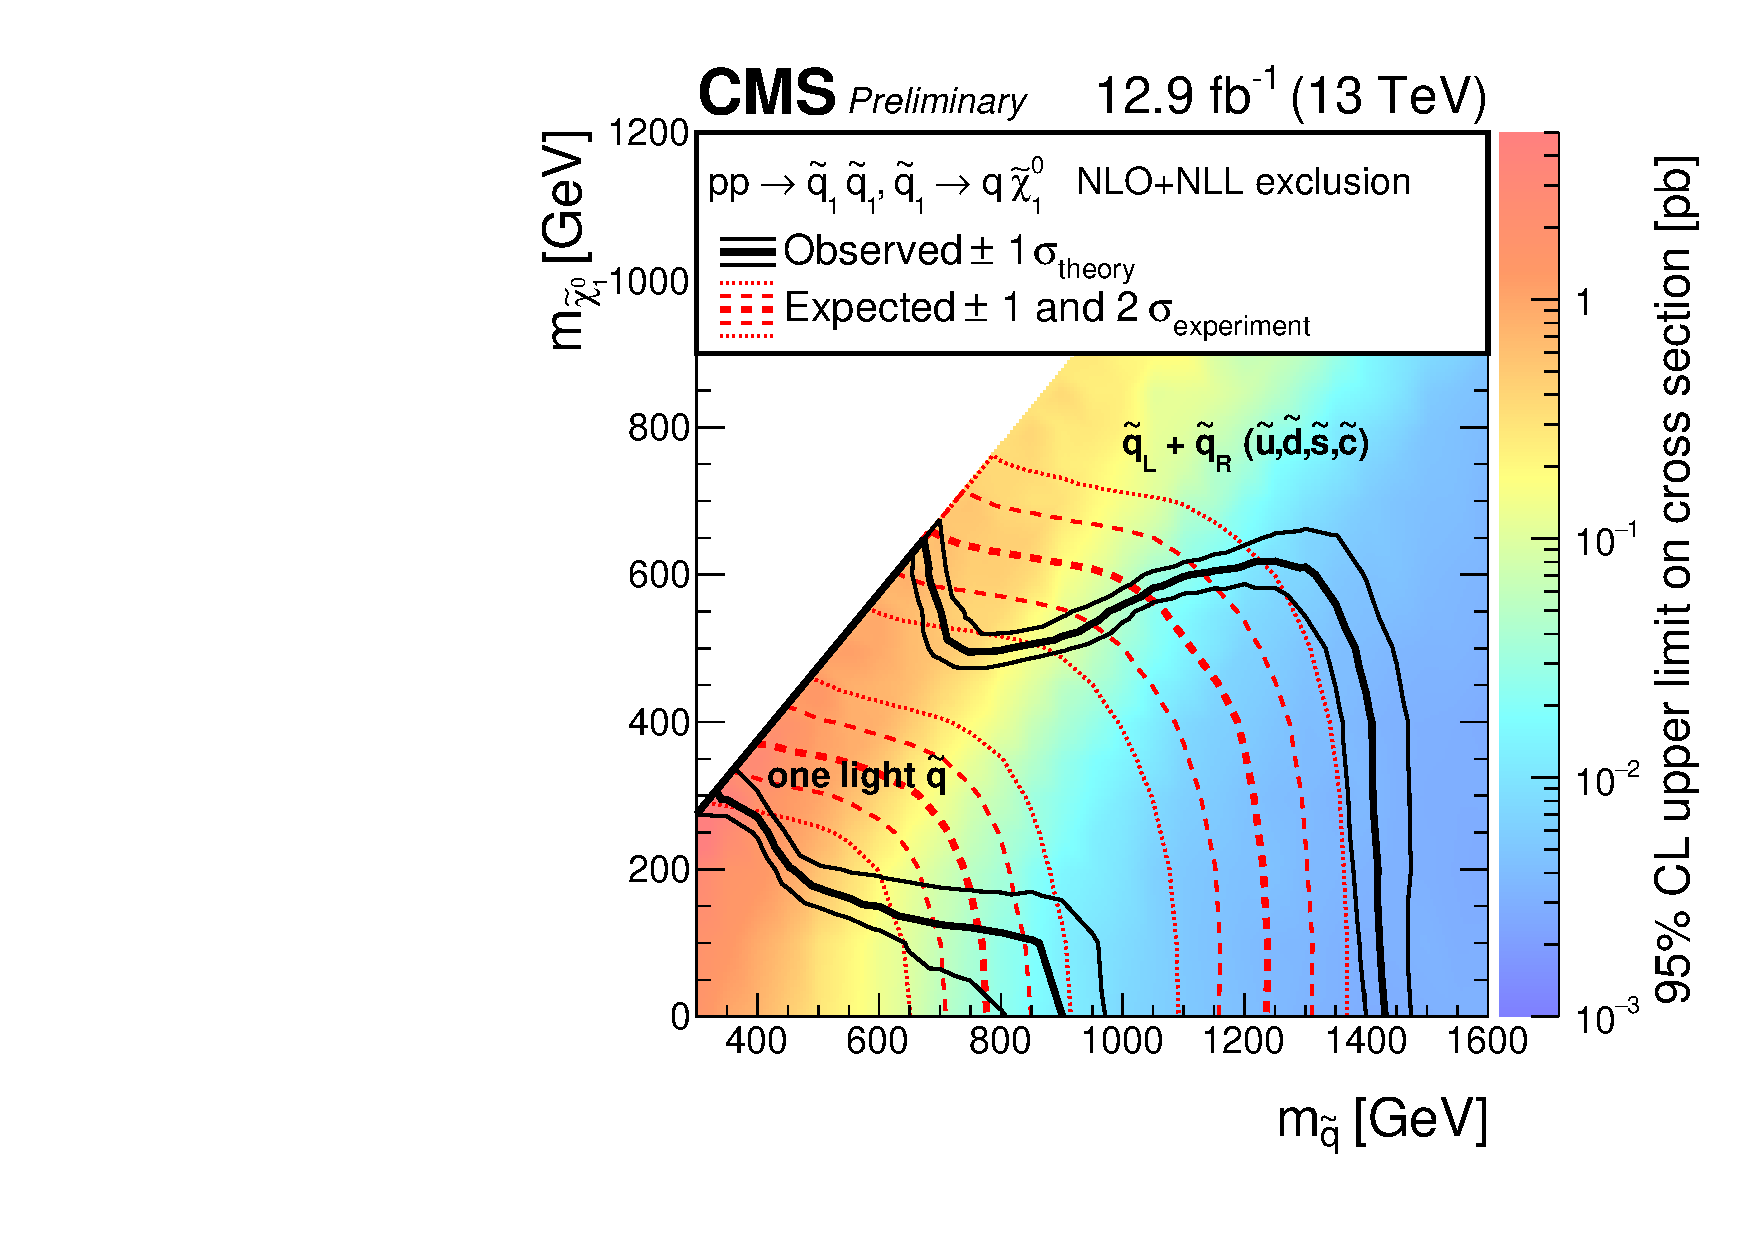
\includegraphics[width=0.5\textwidth]{figs/analysis/interpretation/T2qqXSEC}
%       \label{fig:T2qq_excl}
%     } ~~
%     % \subfloat[T2qq: $\epsilon_{sig}^{\mathrm{4\,cat}}$]{
%     %   \includegraphics[width=0.45\textwidth]{figures/jetRanking/T2qq/eff/T2qq_merging_4_cats}
%     %   \label{fig:T2qq_eff}
%     % } ~~
%     % \subfloat[T2qq: $\epsilon_{sig}^{\mathrm{4\,cat}}/\epsilon_{sig}^{\mathrm{tot}}$]{
%     %   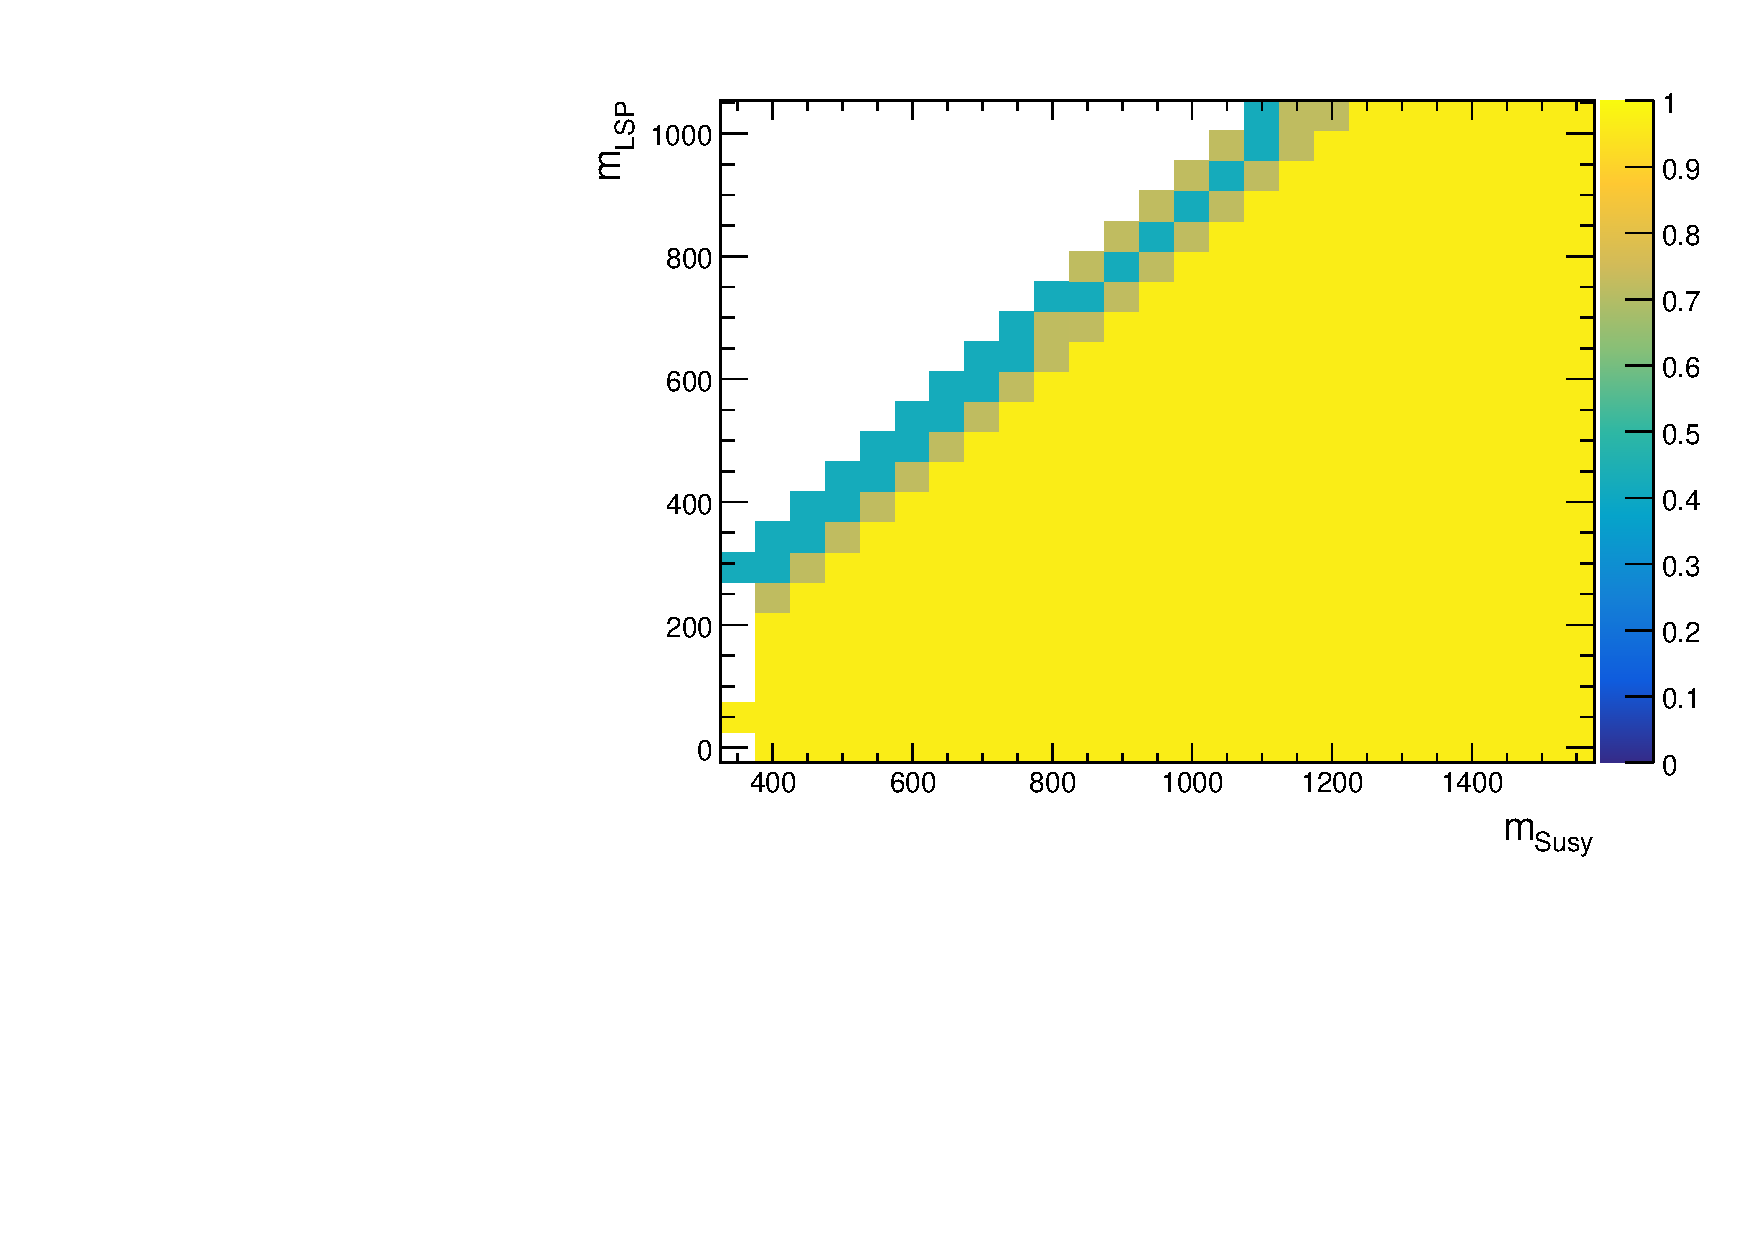
\includegraphics[width=0.45\textwidth]{figures/susyResults/T2qq_doubleRatioAcceptance}
%     %   \label{fig:T2qq_eff_doubleRatio}
%     % }
%     \label{fig:T2qq}
%         \subfloat[T1qqqq: Upper limit on the cross section in the
%     $(m_{\mathrm{Gluino}},m_{\mathrm{\LSP}})$ plane]{
%       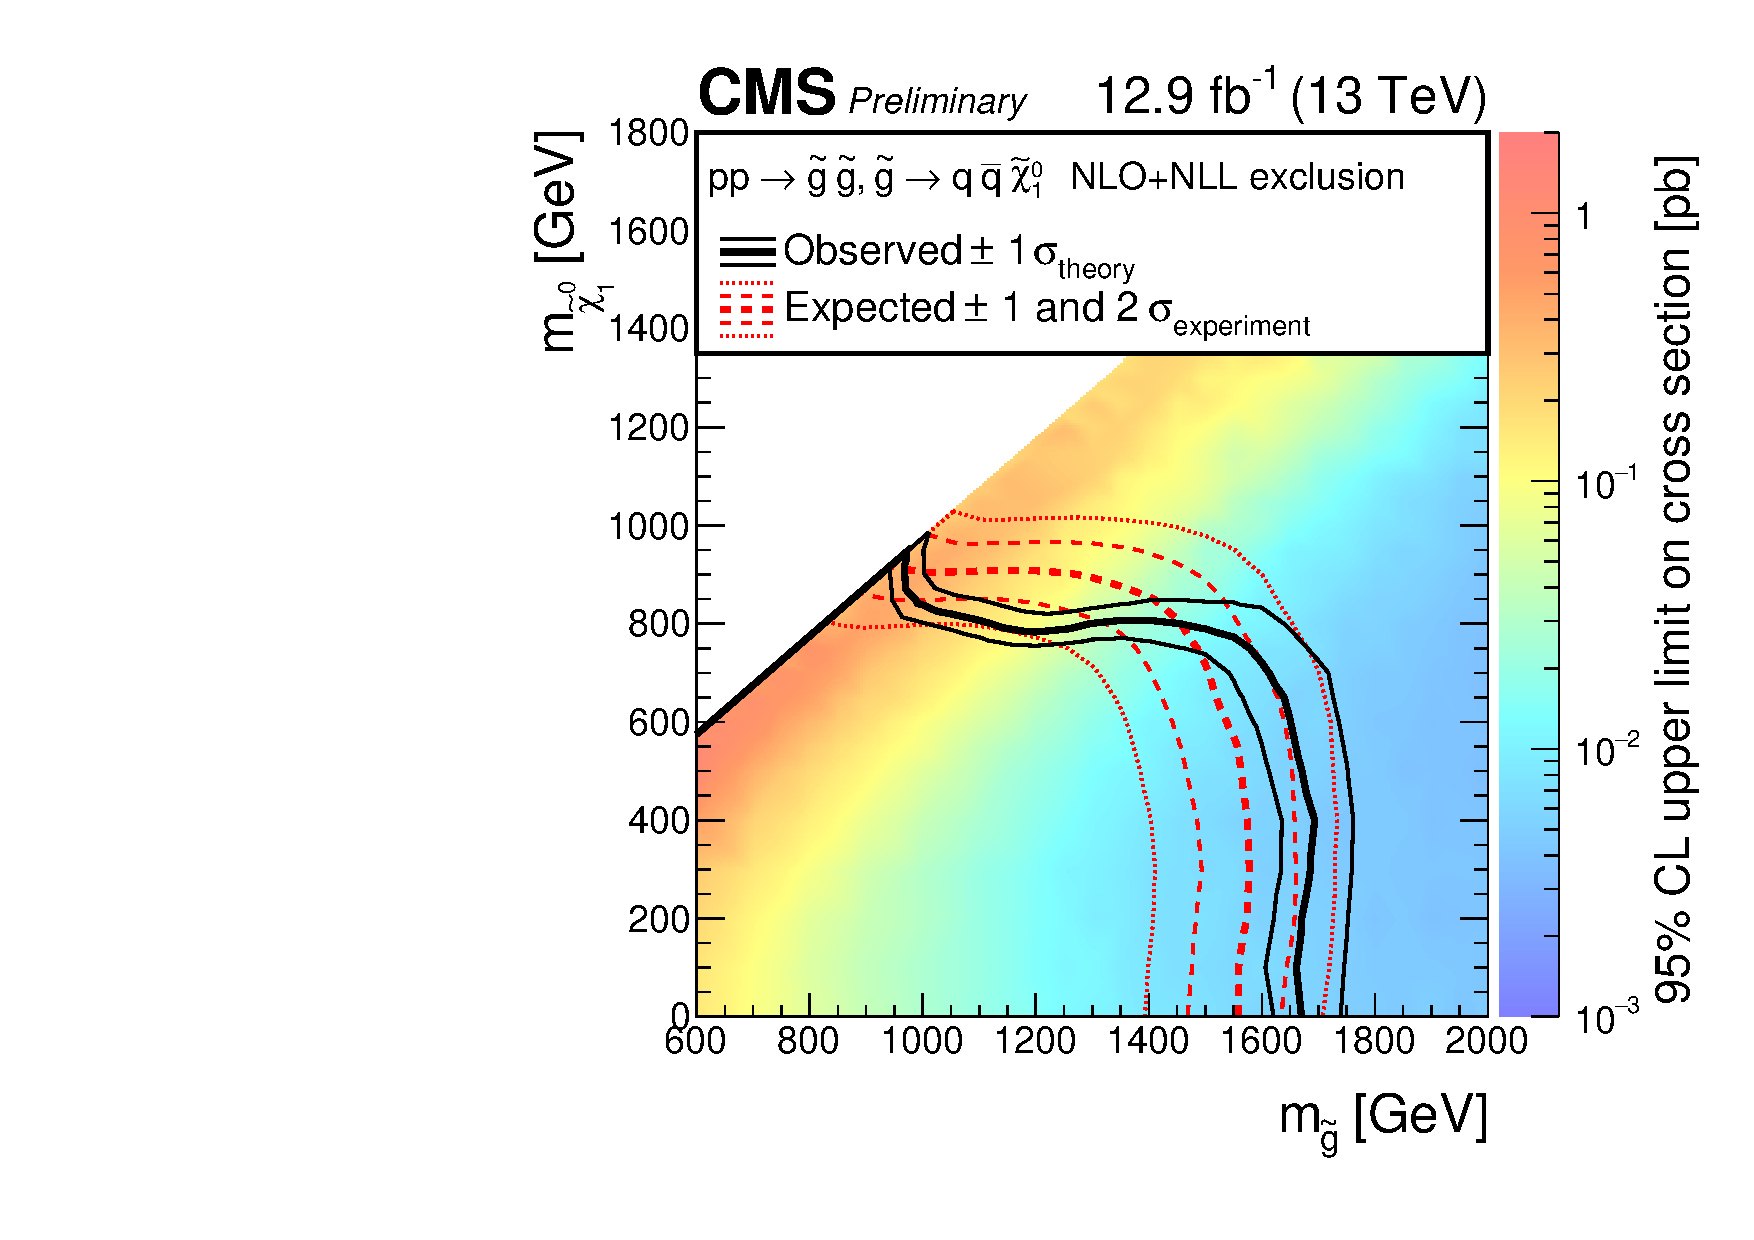
\includegraphics[width=0.5\textwidth]{figs/analysis/interpretation/T1qqqqXSEC}
%       \label{fig:T1qqqq_excl}
%     } \\
%     % \subfloat[T1qqqq: $\epsilon_{sig}^{\mathrm{4\,cat}}$]{
%     %   \includegraphics[width=0.45\textwidth]{figures/jetRanking/T1qqqq/eff/T1qqqq_merging_4_cats}
%     %   \label{fig:T1qqqq_eff}
%     % } ~~
%     % \subfloat[T1qqqq: $\epsilon_{sig}^{\mathrm{4\,cat}}/\epsilon_{sig}^{\mathrm{tot}}$]{
%     %   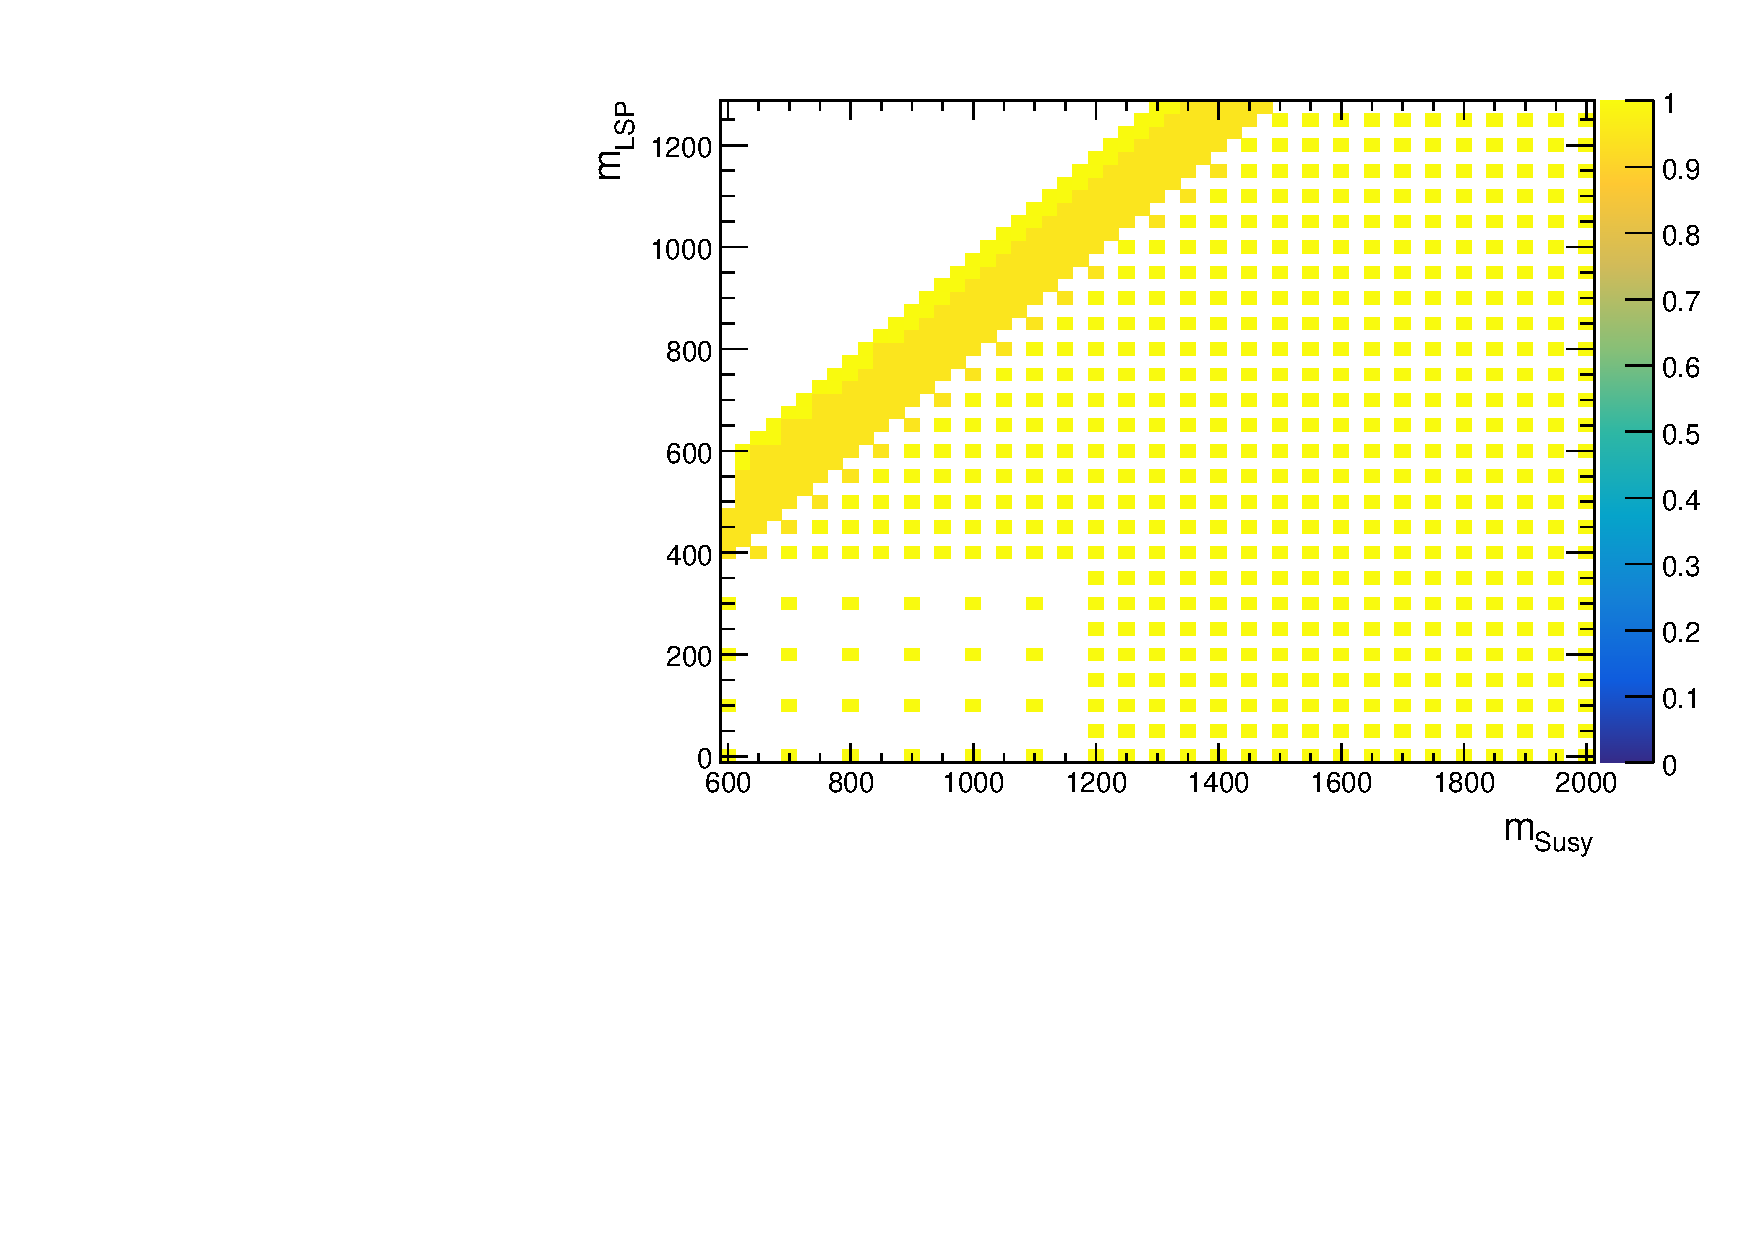
\includegraphics[width=0.45\textwidth]{figures/susyResults/T1qqqq_doubleRatioAcceptance}
%     %   \label{fig:T1qqqq_eff_doubleRatio}
%     % }
%     \caption{
%       The 95\% observed upper limit on the cross section (histogram),
%       with the expected (dotted red line) and observed (black line)
%       exclusion contours. For a selection of \SUSY models discussed in
%       Sec.~\ref{sec:signalModel}.
%       % Bottom right: ratio of the signal acceptance including 4 categories to the acceptance including the whole signal region. 
%     }
%     \label{fig:T1qqqq}
%   \end{center}
% \end{figure}

\newcommand{\ph}{\ensuremath{\phantom{1}}}
\begin{table}[tb]
  \caption{A summary of the strongest observed (expected) mass
  exclusions for the simplified models introduced in
  Sec.~\ref{sec:signalModel}. The limit on the mass of the relevant
  gluino or squark and the \LSP, $\tilde{\chi^0_1}$, are quoted and
  all have uncertainties of $\pm$25\GeV.  
  }
  \label{tab:simplified-models-limits}
  \centering
  \footnotesize
  \begin{tabular}{ llcc }
    \hline
    Production mode & Squark        & \multicolumn{2}{c}{Strongest obs. (exp.) mass exclusion [GeV]}\T\B \\
    \cline{3-4}                     
                    &               & Gluino or squark\T\B & $\tilde{\chi^0}$                                               \\
    \hline                          
    Gluino-mediated & Bottom        & 1775 \ph(1850)       & 1175 \ph(1200)                                      \\ 
    Gluino-mediated & Top           & 1450 \ph(1600)       & \ph750 \ph\ph(800)                                  \\ 
    Direct          & Bottom        & 1025 \ph\ph(975)     & \ph525 \ph\ph(500)                                  \\ 
    Direct\B        & Top           & \ph875 \ph\ph(925)   & \ph350 \ph\ph(350)                                  \\
    \hline
 \end{tabular}
\end{table}
